\documentclass{hipatia}
\usepackage{graphicx}
%\graphicspath{efemerides/}
\title{Eventos DMAT \\ Março a Novembro/24}
\subtitle{Simpósio}
\author{Cristina Lizana, Elaís Cidely, Henrique da Costa e Roberto Sant'Anna}


%\makeindex
\newcommand{\superau}{\textsuperscript{\underline{a}}~}
\newcommand{\superou}{\textsuperscript{\underline{o}}~}
\begin{document}
\setcounter{page}{\simposiopage}
\maketitle

%\printindex

%\tableofcontents
%\addcontentsline
%\addtocontents

\section{Introdução}

Nesta seção \textsc{Simpósio}  faremos uma breve resenha de eventos organizados por membros da comunidade do Departamento de Matemática (DMAT) do Instituto de Matemática e Estatística (IME) da Universidade Federal da Bahia (UFBA) durante o período de março a novembro de 2024. 


%\medskip
%•	2\superou Workshop África e Matemática – 17 a 20/04/2024
%•	Cerimônia de Premiação Regional da OBMEP – 17/06/2024
%•	Cerimônia de Premiação da OBMEP no Colégio Central – 23/07/2024 (esse item pode ser incluso no item anterior)
%•	XXIII EBT – 29/07 a 03/08/2024
%•	XXVII EBP – 05 a 09/08/2024
%•	Workshop 2 + 3 in Dynamics – 16 a 20/09/2024
%•	Prêmio PIBIC T UFBA 2024
%•	Colação de grau 2024.1 – 04/10/2024
%•	Aulão Olímpico: Superando Desafios em Matemática – 17/10/2024
%•	3\superou EBMM – 13 a 16/11/2024
%•	IX EPGMAT – 18 a 22/11/2024
%•	Cerimônia de Premiação da OMEBA – 03/12/2024 (a ocorrer em dezembro!)
%
%
%\newpage

\section{Projeto PECMat}

O projeto de extensão PECMat - ``Projeto Egressos dos cursos de Matemática da UFBA, conectando passado, presente e futuro no IME'' foi criado em novembro de 2023, ano em que os cursos de Graduação em Matemática da UFBA completaram  80 anos.

Criado com o intuito de honrar a história, as  realizações e contribuições do Departamento de Matemática da UFBA, o projeto é coordenado por Elaís Cidely, Elen Deise e Roberto Sant'Anna, todos egressos e atuais professores do DMAT. Elaís Cidely tem bacharelado e mestrado em Matemática pela UFBA e doutorado pelo IMPA; Elen Deise é licenciada em Matemática pela UNEB, com mestrado e doutorado pela UFBA; e Roberto Sant'Anna concluiu a licenciatura, o bacharelado, o mestrado e o doutorado em Matemática pela UFBA. O projeto também encoraja a participação e envolvimento de estudantes atuais dos cursos de Matemática da UFBA. Atualmente, conta com a contribuição de Ravilla Miranda, estudante do curso de licenciatura em Matemática à distância da UFBA, que atua como monitora voluntária no projeto.

\begin{figure}[htb]
    \centering
    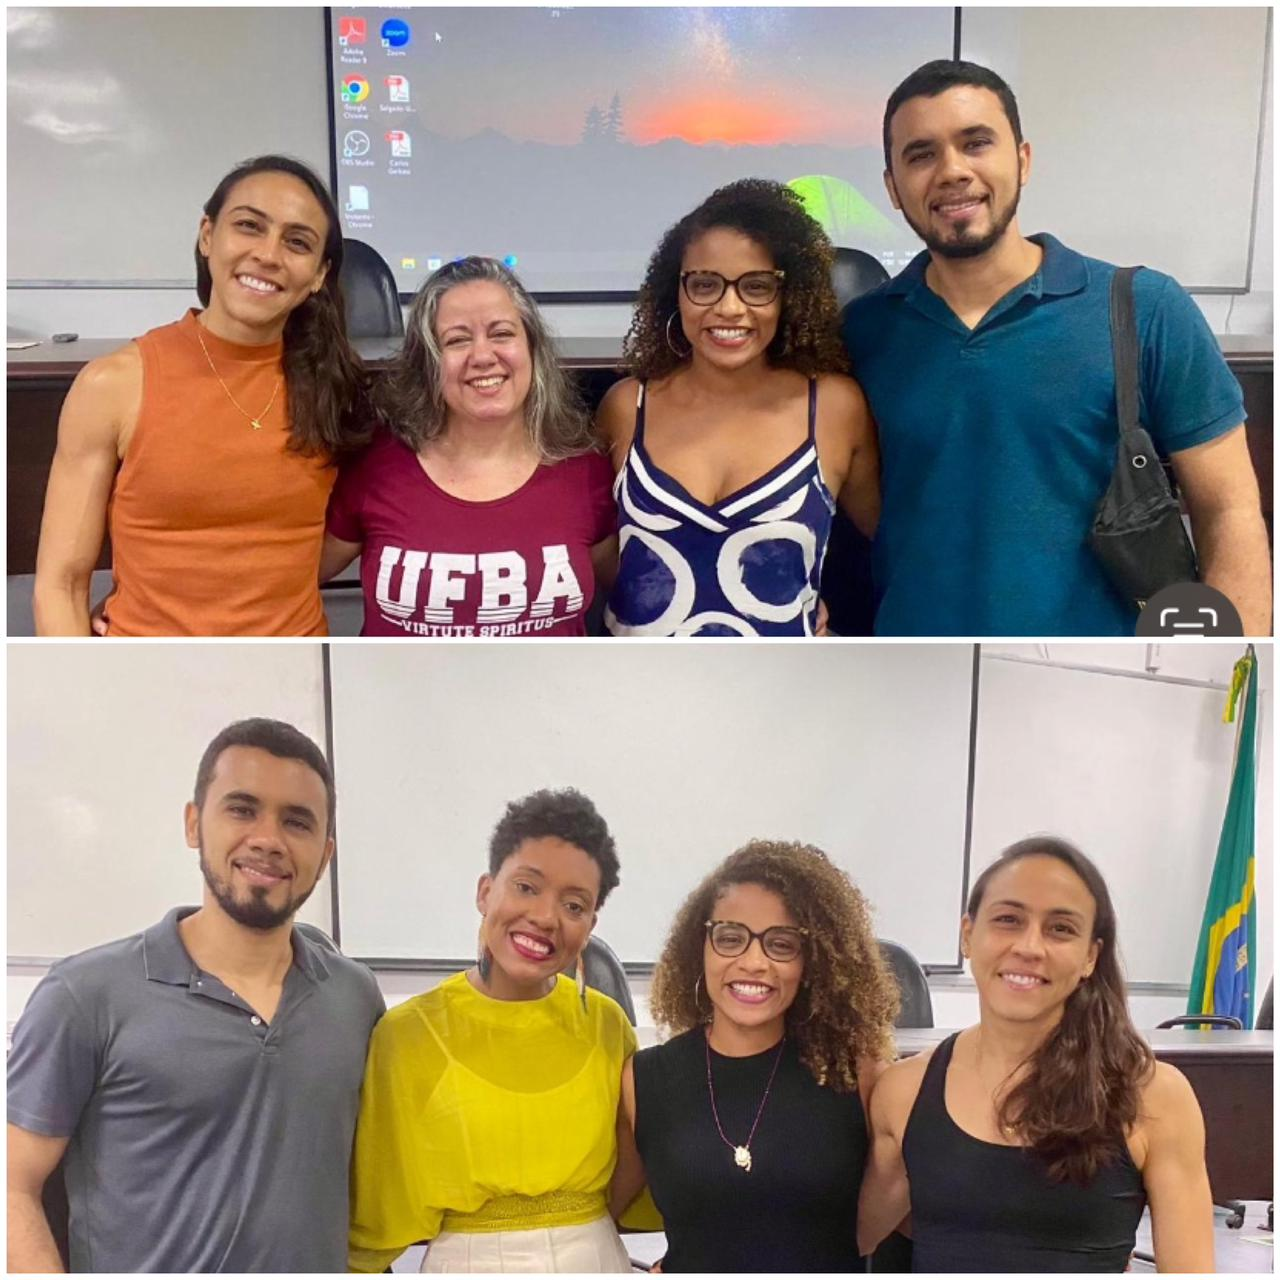
\includegraphics[width=8.5cm]{pecmat1.jpeg}
    \caption{Coordenadores do projeto com as palestrantes Luciana Salgado  e Tamires Purificação, dias 12 de março e 13 de maio de 2024, respectivamente.} %acrescentar o ano?
 \label{PECMat1}
\end{figure}
%
%O projeto também conta atualmente com a contribuição de uma monitora voluntária, estudante do curso de licenciatura em matemática à distância, Ravilla Miranda.
%duplicado

O PECMat busca estabelecer e fortalecer a conexão  entre a comunidade acadêmica do IME, seus egressos e a sociedade em geral. Para isso, as primeiras ações do projeto incluíram a coleta de dados sobre egressos dos cursos de graduação e pós-graduação em Matemática da UFBA.  E a partir de março de 2024, o projeto passou a realizar diversas palestras no auditório do IME, ministradas por egressos do IME que hoje atuam em diferentes instituições, como UFBA, UFRJ, IFBaiano e USP/UFSCar. Na ocasião, eles compartilham e divulgam sobre seus projetos, suas trajetórias e suas experiências acadêmicas e profissionais com outros egressos e atuais docentes e discentes da UFBA e outras instituições. Essas palestras contribuem de forma significativa para a formação dos nossos atuais estudantes.
%trocar "futuros egressos" por 'atuais estudantes'? a palavra egresso foi repetida algumas vezes

Entre os palestrantes, destacam-se  matemáticos com longa trajetória em suas carreiras, como Luciana Salgado (UFRJ), Evandro Santos (UFBA), Graça Luzia (UFBA), Carlos Bahiano (UFBA) e Manuela Souza (UFBA), além de jovens pesquisadores como Tamires Purificação (UFRJ), Leandro Teixeira (IFBaiano) e Fernando Moraes (USP/UFSCar).

Ao final de cada palestra, acontece o tradicional sorteio de um livro entre os participantes do auditório, além do \textit{coffee break}, que serve como mais uma oportunidade única de interação entre membros internos e externos à comunidade do IME e os nossos egressos.

\begin{figure}[htb]
    \centering
    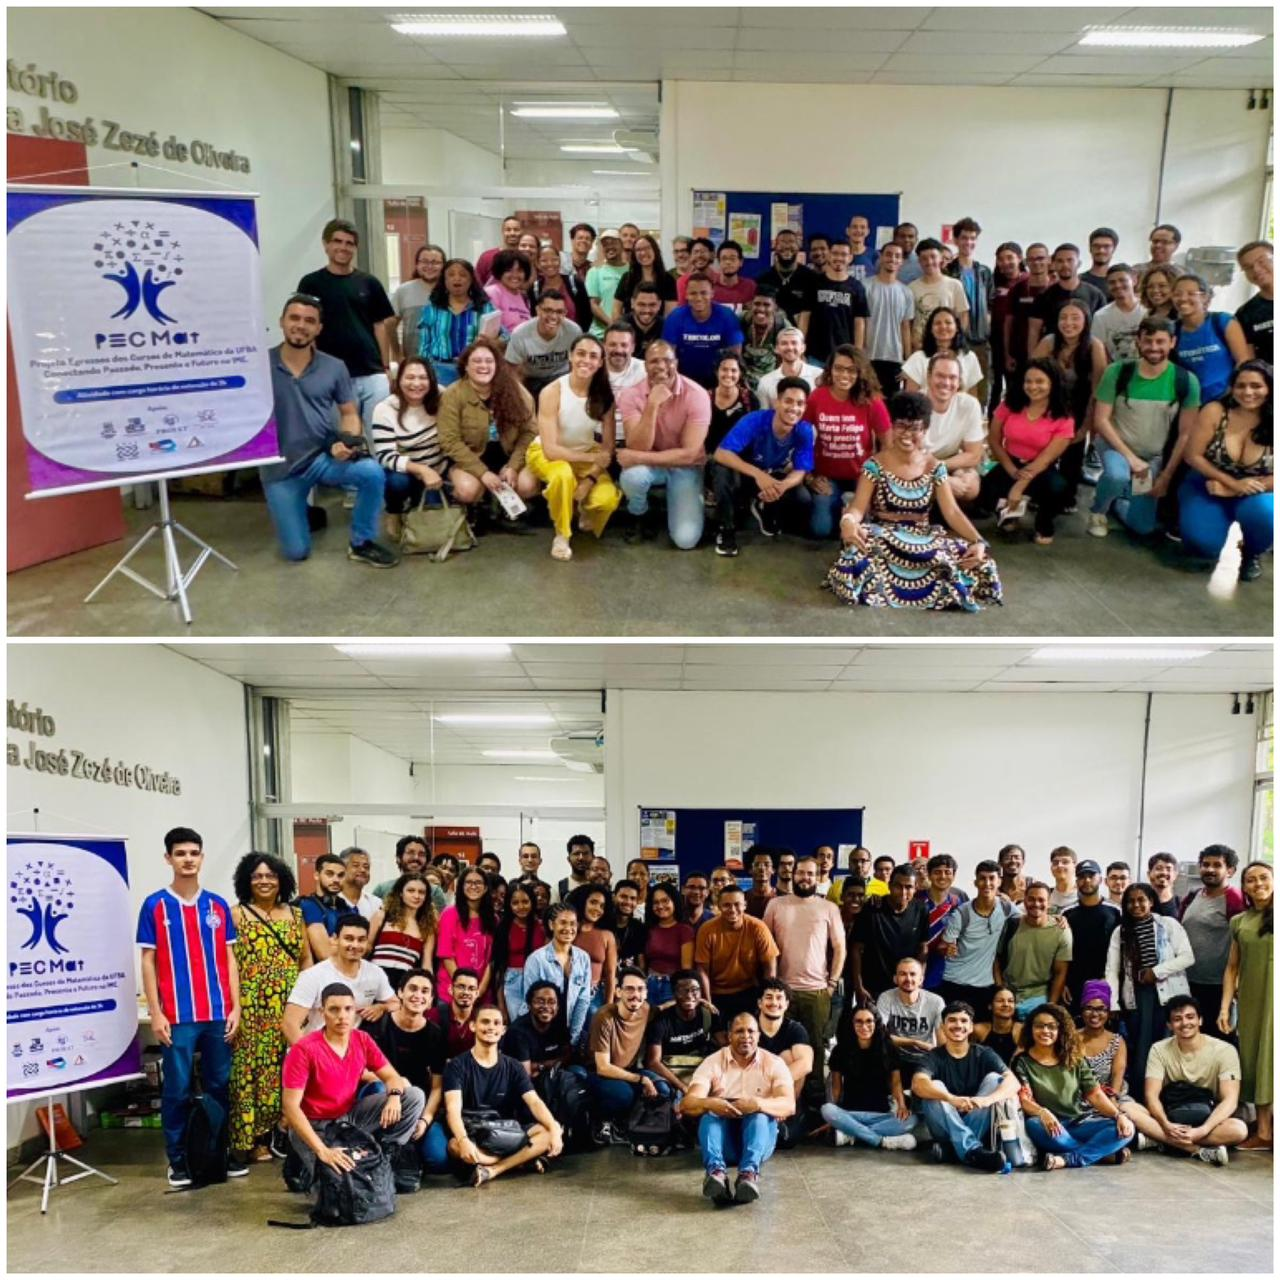
\includegraphics[width=8.5cm]{pecmat2.jpeg}
    \caption{Participantes ao final das palestras dos professores Manuela Souza e Carlos Bahiano, dias 20 de agosto e 17 de outubro de 2024, respectivamente.}
 \label{PECMat2}
\end{figure}

Além disso, para ampliar o alcance dessa importante troca de conhecimentos entre diferentes gerações de matemáticos, as gravações das palestras são disponibilizadas no canal do DMAT no YouTube (\href{http://www.youtube.com/@dmatufba}{@dmatufba}), possibilitando que o público externo da UFBA também tenha acesso ao conteúdo.
%adicionar o link do canal??

Além dos já tradicionais convites a egressos para realizarem palestras no IME, o projeto também pretende realizar outras atividades, como Mesas de Discussão, Encontro de Egressos e Oficinas.
 
Por fim, um dos desafios desta iniciativa é aprimorar as ferramentas para coletar e organizar de forma eficiente os dados sobre os discentes que passaram pelo IME: além de contribuir com a nossa instituição, este mapeamento poderá nos ajudar a alcançar e realizar atividades com um número cada vez maior de egressos ao redor de todo Brasil e do mundo. Portanto, se você é egresso do IME - UFBA e quer ajudar a fortalecer essa rede de conexões e histórias, entre em contato com a coordenação do projeto!

Para mais informações, acesse o instagram do DMAT: \href{https://www.instagram.com/dmatufba?igsh=MXJ0NDVjaThwc2IwMQ==}{@dmatufba}.

\section{2\superou Workshop África e Matemática: Conexões com aporte para o ensino } 

O segundo volume da Revista de Matemática Hipátia apresentou o coletivo Ondjango Asili, reconhecido por suas ações significativas na UFBA e em escolas de Educação Básica de Salvador e região metropolitana. Após o sucesso do ``1\superou Workshop África e Matemática: Conexões com aporte para o ensino'', realizado remotamente em 2022, o coletivo trouxe para os espaços da universidade o ``2\superou Workshop África e Matemática: Conexões com aporte para o ensino'', realizado de 17 a 20 de abril de 2024.

\begin{figure}[htb]
    \centering
    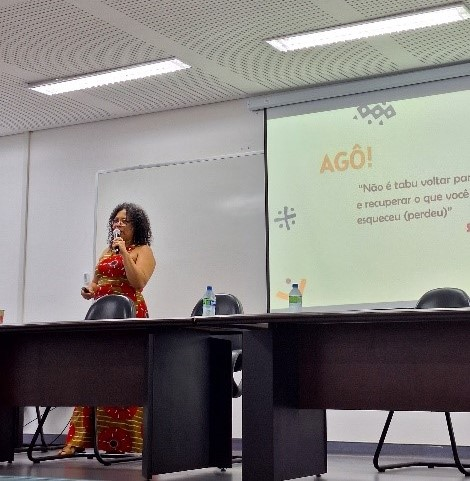
\includegraphics[width=8.5cm]{WAM1.jpg}
    \caption{Professora Simone Moraes.}
 \label{WAM1}
\end{figure}

O evento contou com uma programação diversa, iniciada com a palestra ``Ondjango Asili - Jogos e elementos culturais africanos no ensino de Matemática'', ministrada pela coordenadora do coletivo, Prof.\superau Simone Moraes, no auditório do IME-UFBA. Mesmo local em que foi realizada uma inspiradora roda de conversa sobre ``A experiência da disciplina ACCS \textit{Cultura e Jogos Africanos no Ensino da Matemática}'', envolvendo estudantes do curso de Licenciatura em Matemática da UFBA que cursaram a referida disciplina no segundo semestre de 2023. Esse momento propiciou trocas enriquecedoras e reflexões sobre práticas pedagógicas inovadoras, no contexto da Lei 10.639/03, conectando experiências acadêmicas e culturais.

\begin{figure}[htb]
    \centering
    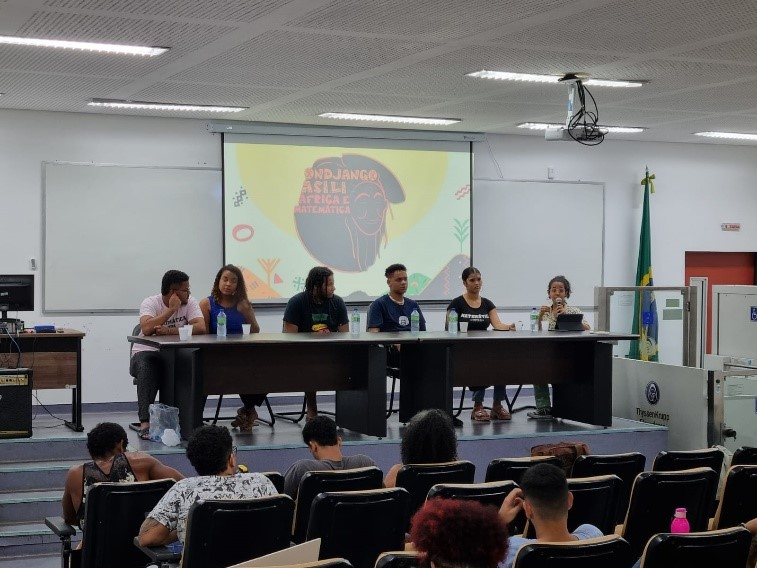
\includegraphics[width=8.5cm]{WAM2.jpg}
    \caption{Estudantes na mesa de discussão ``A experiência da disciplina ACCS Cultura e Jogos Africanos no Ensino da Matemática''.}
 \label{WAM2}
\end{figure}

No \textit{workshop} foram promovidas atividades que aliaram aprendizado e lazer, como oficinas e torneios de jogos africanos de tabuleiros quadriculados e da família mancala. A programação incluiu ainda uma sessão de pôsteres no saguão do IME, na qual bolsistas e estudantes do projeto apresentaram trabalhos desenvolvidos no projeto e na disciplina ACCS, ressaltando o vínculo entre universidade e escolas da Educação Básica.

\begin{figure}[htb]
    \centering
    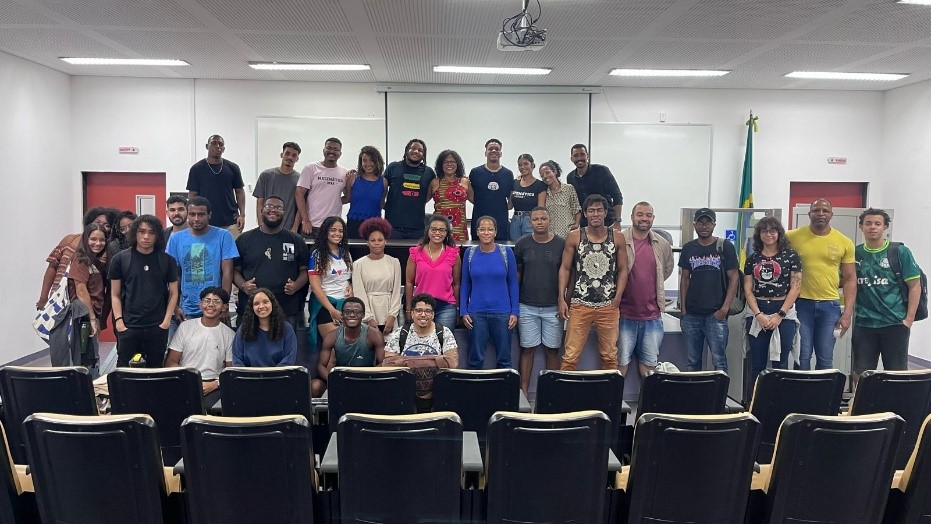
\includegraphics[width=8.5cm]{WAM3.jpg}
    \caption{Participantes do primeiro dia do Workshop.}
 \label{WAM3}
\end{figure}

No último dia do evento, houve uma exposição das oficinas realizadas na disciplina \textit{Cultura e Jogos Africanos no Ensino da Matemática}, destacando os resultados obtidos pelos estudantes, as atividades criadas na disciplina e as aplicações em escolas públicas de Salvador e região metropolitana. Em seguida, no auditório da FACOM, ocorreu uma mesa de discussão intitulada ``A experiência de participar do PAPIC-EF, Programa de Apoio a Projetos e Iniciação Científica em Matemática'', com os professores Henrique Santiago, Marcus Vinicius Lopes e Susana Quirino, na qual compartilharam com a audiência os impactos da participação neste programa.

\begin{figure}[htb]
    \centering
    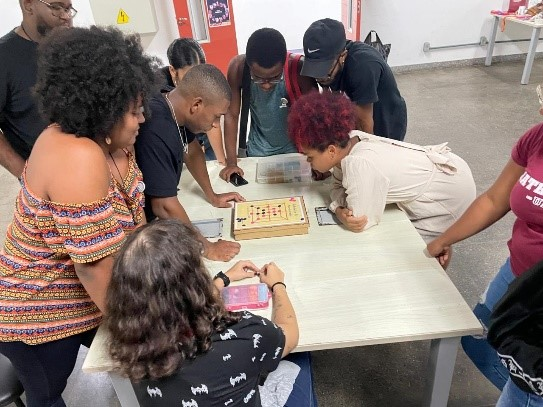
\includegraphics[width=8.5cm]{WAM4.jpg}
    \caption{Torneio de jogos africanos.}
 \label{WAM4}
\end{figure}

O ``2\superou Workshop --- África e Matemática'' reafirmou a importância do Ondjango Asili e suas contribuições para um ensino de Matemática mais inclusivo, conectando Matemática e África, através da valorização da cultura e dos saberes africanos como elementos transformadores no processo de ensino e aprendizagem.


%O segundo volume da Revista de Matemática Hipátia apresentou o coletivo Ondjango Asili, reconhecido por suas ações significativas na UFBA e em escolas de Educação Básica de Salvador. Após o sucesso do 1\superou Workshop África e Matemática, realizado virtualmente em 2022, o coletivo trouxe para os espaços da universidade o "2\superou Workshop África e Matemática: Conexões com aporte para o ensino", entre os dias 17 e 20 de abril.

%O evento contou com uma diversa programação, iniciada com a palestra "Ondjango Asili - Jogos e elementos culturais africanos no ensino de matemática", ministrada pela coordenadora do coletivo, Prof.\superau Simone Moraes, no auditório do IME-UFBA. Mesmo local em que foi realizada uma inspiradora roda de conversa sobre "A experiência da disciplina ACCS cultura e jogos africanos no ensino de matemática", envolvendo estudantes do curso de licenciatura em matemática da UFBA. Este momento propiciou trocas enriquecedoras e reflexões sobre práticas pedagógicas inovadoras, conectando experiências acadêmicas e culturais.

%Além disso, o workshop promoveu atividades que aliaram aprendizado e lazer, como oficinas e torneios de jogos africanos de tabuleiros quadriculados e da família manca. A programação incluiu ainda uma sessão de pôsteres no saguão do IME, onde estudantes bolsistas apresentaram trabalhos desenvolvidos na disciplina ACCS, ressaltando o vínculo entre universidade e escolas da Educação Básica.

%No último dia do evento, houve uma exposição das oficinas realizadas na disciplina Cultura e Jogos Africanos no Ensino da Matemática, destacando os resultados obtidos pelos estudantes e as atividades desenvolvidas ao longo do curso. E em seguida, no auditório da FACOM, ocorreu uma mesa de discussão especial intitulada "A experiência de participar do PAPIC-EF, Programa de Apoio a Projetos e Iniciação Científica em Matemática", com os professores Henrique Santiago, Marcus Vinicius Lopes e Susana Quirino. O dia foi encerrado com a cerimônia oficial de conclusão do workshop, celebrando as trocas e aprendizagens promovidas pelo evento.  

%Esse 2\superou Workshop reafirmou a importância do Ondjango Asili e suas contribuições para a construção de uma educação matemática básica mais inclusiva, ao valorizar a cultura e os saberes africanos como elementos transformadores no processo de ensino e aprendizagem.


%\section{Cerimônia de Premiação da OBMEP}  %Roberto


%Cerimônia de Premiação da OBMEP: Celebrando o Brilho dos Jovens Matemáticos

%Imagem representativa da Cerimônia. %?

%O Salão Nobre da Reitoria da UFBA foi palco de uma bela celebração da matemática no dia 17 de junho. A Cerimônia de Premiação da 18\superau OBMEP (2023) reuniu alunos medalhistas de ouro, prata e bronze de Salvador e Região Metropolitana, seus familiares, professores e convidados, em um evento que reconheceu e celebrou o talento e a dedicação desses jovens.

%A cerimônia contou com a presença ilustre do Reitor Paulo Cesar Miguez de Oliveira, que parabenizou os alunos e destacou a importância da OBMEP na formação educacional, incentivando o desenvolvimento do raciocínio lógico e a paixão pela matemática. O evento também foi abrilhantado pela participação do Duo VibraCor, formado pelos professores da UFBA Ricardo Camponogara e Aquim Sacramento, que encantou a todos os mais de 200 presentes com belas músicas.

%Imagem da banda musical. %?

%Entre as presenças importantes, estavam o professor Kleyber Mota, Diretor do IME-UFBA, o Coordenador Regional da OBMEP, professor Roberto Sant'Anna, e representantes da sociedade civil ligados à educação, como a Sra. Rosilene Cavalcante, da SEC-BA, o Sr. Isnard Araújo, vereador de Salvador, a Sra. Isabela Cavalcanti, da SMED-Salvador, e a Sra. Patrícia Ribeiro, do NTE 26.

%Imagem da mesa principal da cerimônia. %?

%Também estiveram presentes, além dos medalhistas, pais, amigos e os professores dos homenageados, com os quais puderam compartilhar belas memórias, quer seja na caminhada rumo à medalha, quer seja nos momentos da chegada ao pódio.

%A Cerimônia de Premiação da OBMEP foi um momento de grande inspiração para os jovens talentos da matemática, que receberam suas medalhas com orgulho e entusiasmo, compartilhando experiências e motivando uns aos outros em suas jornadas de aprendizado.

%Imagem de colocação de medalha. %?

%Para mais informações sobre as ações da OBMEP em Salvador e Região Metropolitana, visitem o perfil do projeto Matemática Olímpica no Instagram, \href{https://www.instagram.com/mat.olimpica/#}{@mat.olimpica}!



\section{XXIII Encontro Brasileiro de Topologia} %~Henrique

%O XIII Encontro Brasileiro de Topologia aconteceu de 29 de julho a 03 de agosto de 2024 no IME-UFBA e reuniu pesquisadores, professores e alunos de variadas regiões do Brasil, além de uma boa quantidade de estrangeiros.
%
%O principal objetivo do EBT é divulgar os recentes avanços da área de Topologia, além de estabelecer novas colaborações para novos projetos de pesquisa.
%
%A programação do EBT contou 4 mini-cursos (2 básicos e 2 avançados), 20 palestras, 25 comunicações-curtas e apresentação de 40 pôsteres. 
%
%Mais informações sobre o XXIII EBT podem ser encontradas em \href{https://xxiiiebt.ime.ufba.br}{https://xxiiiebt.ime.ufba.br} 
%
%A XXIV edição do EBT ocorrerá em 2026 na UFES, Vitória.

O XXIII Encontro Brasileiro de Topologia aconteceu de 29 de julho a 03 de agosto de 2024 no IME-UFBA (Fig. \ref{EBT}).
O evento bienal é tradição no calendário da Matemática: desde 1979 vem reunindo pesquisadores, professores e alunos de variadas regiões do Brasil e do exterior. Os principais tópicos que têm sido abordados são: folheações, ações localmente livres de grupos, cohomologia limitada, classes características, grupos de bordismo, singularidades, teoria de ponto fixo e outros tópicos na interface da Topologia Algébrica e Diferencial.

Neste ano foram realizados 4 mini-cursos (2 básicos e 2 avançados), 20 palestras, 25 comunicações-curtas e apresentação de 40 pôsteres, além da promoção de um evento satélite, o 1\superou Workshop Invernal de Topologia e Teoria dos Conjuntos (WITTC) da UESC, na Universidade de Santa Cruz, realizado entre os dias 5 e 7 de agosto de 2024 em Ilhéus-BA.

Os principais objetivos do EBT são divulgar os recentes avanços da área de Topologia e fomentar e fortalecer novas colaborações para projetos de pesquisa, criando elos entre brasileiros e estrangeiros.

Mais informações sobre o XXIII EBT podem ser encontradas em \href{https://xxiiiebt.ime.ufba.br}{https://xxiiiebt.ime.ufba.br}.
Informações gerais sobre o EBT podem ser encontradas na página  \href{https://www.dm.ufscar.br/profs/ebt/about.php}{https://www.dm.ufscar.br/profs/ebt}.

A XXIV edição do EBT ocorrerá em 2026 na UFES, Vitória-ES.

\begin{figure}[htb]
    \centering
    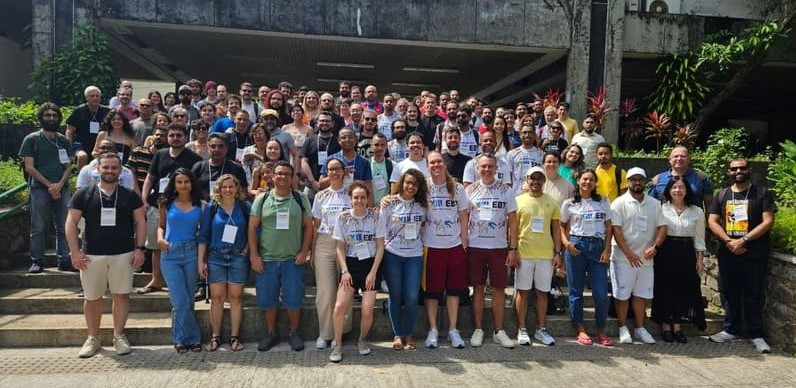
\includegraphics[width=8.5cm]{EBT.jpeg}
    \caption{Participantes no XIII Encontro Brasileiro de Topologia.}
 \label{EBT}
\end{figure}

%%%%%%%%%%%%%%%%%%%%%%%%%%%%%%%%%%%%%%%%%%%%%%%%%%%%%%%%%%%%%%%%%%%%%%%%%%%%%%%%%%%%%%%
\section{27\superau Escola Brasileira de Probabilidade} %~Henrique => apenas editei o texto, não sei quem foi que escreveu a princípio...
%A Escola Brasileira de Probabilidade é, sem dúvida, um dos eventos mais importantes no mundo na nossa área de pesquisa. A 27\superau edição deste ano ocorreu em Salvador, Bahia, de 05 a 09 de agosto de 2024. Esta foi apenas a segunda vez que o evento foi realizado na região nordeste do país e a primeira vez na Bahia.
%\begin{figure}[htb]
%    \centering
%    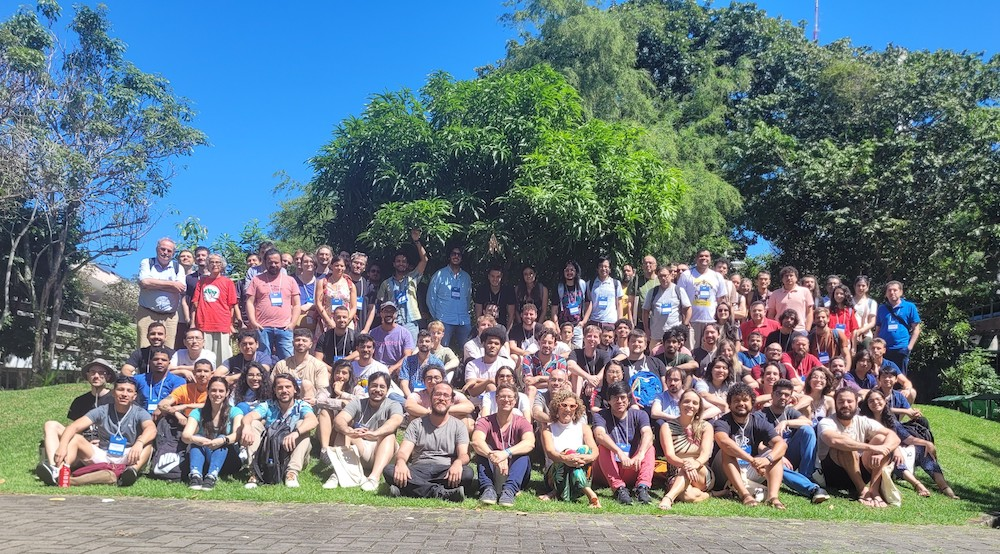
\includegraphics[width=8cm]{EBP.jpg}
%    \caption{Participantes na 27\superau Escola Brasileira de Probabilidade.}
% \label{EBP}
%\end{figure}
%
%Ao todo, 109 estudantes, jovens pesquisadores e professores participaram do evento, representando uma ampla diversidade de países, como Brasil, Argentina, Peru, Chile, Uruguai, Estados Unidos, Holanda, Itália, Reino Unido, Alemanha, França, Suíça, China e Coreia do Sul. Esse panorama internacional destaca a relevância do evento para a nossa área de estudo. A programação incluiu dois minicursos, oito palestras plenárias, cinco palestras curtas e várias sessões de pôsteres. Os minicursos foram conduzidos por Frank den Hollander (Leiden University, Holanda), abordando avanços recentes em sistemas de partículas interagentes em grafos, e por Alessandra Ciprian (University College London, Reino Unido), que tratou do Cálculo Grassmanniano na Teoria da Probabilidade. As palestras plenárias foram ministradas por Hubert Lacoin (IMPA, Brasil), Gioia Carinci (Università di Modena e R. Emilia, Itália), Leonardo Rolla (USP, Brasil), Marielle Simon (Université Lyon 1, França), Alexandre Stauffer (King's College London, Reino Unido), Inés Armendariz (Universidad de Buenos Aires, Argentina), Franco Severo (ETH Zuerich, Suíça) e Lisa Hartung (Universitaet Mainz, Alemanha). Além disso, os jovens pesquisadores emergentes que tiveram a oportunidade de apresentar palestras curtas foram Chiara Franceschini (Università di Modena e R. Emilia, Itália), Carla Crucianelli (Princeton, Estados Unidos), Daniel Yukimura (IMPA, Brasil), Angeliki Koutsimpela (Universitaet Augsburg, Alemanha), e María Cecilia de Vita (Universidad de Buenos Aires, Argentina).
%
%Finalmente, o evento também contou com momentos de confraternização, como um coquetel no primeiro dia e um jantar de encerramento, proporcionando um ambiente propício para a socialização e o fortalecimento de laços entre os participantes.
%
%Mais informações sobre a escola podem ser achados no site \href{https://ebp.ufba.br/}{https://ebp.ufba.br/}
%

A Escola Brasileira de Probabilidade é, sem dúvida, um dos eventos mais importantes no mundo nessa área de pesquisa. 
A 27\superau edição deste ano ocorreu em Salvador, Bahia, de 05 a 09 de agosto de 2024 (Fig. \ref{EBP}). 
Essa foi apenas a segunda vez que o evento foi realizado na região nordeste do país e a primeira vez na Bahia.
\begin{figure}[htb]
    \centering
    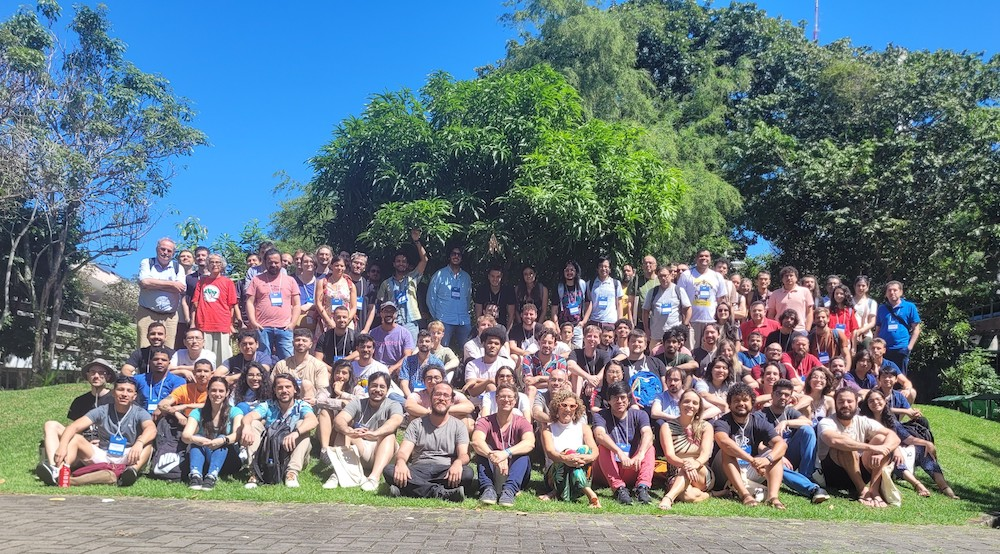
\includegraphics[width=8.5cm]{EBP.jpg}
    \caption{Participantes na 27\superau Escola Brasileira de Probabilidade.}
 \label{EBP}
\end{figure}

Ao todo, 109 estudantes, jovens pesquisadores e professores participaram do evento, representando uma ampla diversidade de países, como Brasil, Argentina, Peru, Chile, Uruguai, Estados Unidos, Holanda, Itália, Reino Unido, Alemanha, França, Suíça, China e Coreia do Sul. 
Esse panorama internacional destaca a relevância do evento para a área de estudo. 

A programação incluiu dois minicursos, oito plenárias, cinco comunicações curtas e várias sessões de pôsteres. 
Os minicursos foram conduzidos por Frank den Hollander (Leiden University, Holanda), abordando avanços recentes em sistemas de partículas interagentes em grafos, e por Alessandra Ciprian (University College London, Reino Unido), que tratou do Cálculo Grassmanniano na Teoria da Probabilidade. 
As palestras plenárias foram ministradas por Hubert Lacoin (IMPA, Brasil), Gioia Carinci (Università di Modena e R. Emilia, Itália), Leonardo Rolla (USP, Brasil), Marielle Simon (Université Lyon 1, França), Alexandre Stauffer (King's College London, Reino Unido), Inés Armendariz (Universidad de Buenos Aires, Argentina), Franco Severo (ETH Z\"{u}rich, Suíça) e Lisa Hartung (Universitaet Mainz, Alemanha). 
Além disso, jovens pesquisadores também tiveram a oportunidade de apresentar palestras curtas sobre seus tópicos de interesse.
%foram Chiara Franceschini (Università di Modena e R. Emilia, Itália), Carla Crucianelli (Princeton, Estados Unidos), Daniel Yukimura (IMPA, Brasil), Angeliki Koutsimpela (Universitaet Augsburg, Alemanha), e María Cecilia de Vita (Universidad de Buenos Aires, Argentina).

Finalmente, o evento também contou com momentos de confraternização, como um coquetel no primeiro dia e um jantar de encerramento, proporcionando um ambiente propício para a socialização e o fortalecimento de laços entre os participantes.

Mais informações sobre a escola podem ser encontradas no site \href{https://ebp.ufba.br/}{https://ebp.ufba.br}.

%%%%%%%%%%%%%%%%%%%%%%%%%%%%%%%%%%%%%%%%%%%%%%%%%%%%%%%%%%%%%%%%%%%%%%%%%%%%%%%%%%%%%%%


\section{Prêmio PIBIC$\&$T UFBA 2024} % (Cris)



O Prêmio UFBA PIBIC$\&$T 2024 é oferecido pela Pró-Reitoria de Pesquisa e Pós-Graduação da  Universidade Federal da Bahia aos trabalhos selecionados pelos Comitês Interno e Externo do Programa Institucional de Bolsas de Iniciação Científica no ciclo do edital PIBIC$\&$T 2022-2023.

A Bacharel em Matemática,  Gabriela Kipper Paim, ex-aluna de nossos cursos de Matemática, recebeu uma  menção honrosa na área de Ciências Exatas e da Terra pelo trabalho desenvolvido no Programa de Iniciação Científica 2022-2023, sob a orientação da professora Cristina Lizana Araneda.

A cerimônia de entrega do prêmio aconteceu no dia 12 de setembro de 2024, no Salão Nobre da Reitoria (Fig. \ref{premio}).  A palestra de abertura foi proferida pela professora Helena Nader, Presidente da Academia Brasileira de Ciências, com o título ``A importância da Iniciação Científica para a Pesquisa Brasileira'', destacando o papel fundamental da iniciação científica no desenvolvimento da pesquisa no país.

 Foi um momento festivo, com a UFBA reconhecendo a excelência de seus bolsistas e orientadores de Iniciação Científica e Tecnológica, marcando o início do novo ciclo 2024-2025.


\begin{figure}[htb]
    \centering
    \includegraphics[width=8.5cm]{PIBIC3.jpg}
    \caption{Cerimônia de Premiação.}
 \label{premio}
\end{figure}

%O nosso programa de Pós-graduação em Matemática foi agraciado com duas menções honrosas: Juan Carlos Arroyave Blanco (Dissertação 2021), orientado pelo prof. Tertuliano Franco; e Elivan Neri Lima (Dissertação 2022), orientado pela prof.\superau Cristina Lizana Araneda. Foi realizada uma cerimônia de 
%premiação dos trabalhos (Fig. \ref{premio}), celebrando o encerramento deste primeiro Prêmio UFBA de Tese, 
%Dissertação Acadêmica e Trabalho de Conclusão de Programa Profissional,  no Salão Nobre da Reitoria no dia 12 de dezembro de 2023.

Para mais informações sobre a Pró-Reitoria de Pesquisa e Pós-Graduação (PRPPG) acesse
 \href{https://prppg.ufba.br/}{https://prppg.ufba.br/}, ou sobre o Programa de Pós-graduação em Matemática da UFBA acesse \href{https://pgmat.ufba.br/}{https://pgmat.ufba.br/}.
 

%\newpage

\section{Workshop 2+3 in Dynamics - Joint 2nd Workshop Nordestino de Sistemas Dinâmicos and 3rd Jangada Dinâmica}

%Workshop 2+3 in Dynamics: Uma união frutífera em Sistemas Dinâmicos no Nordeste

%Incluir alguma imagem aqui

Entre os dias 16 e 20 de setembro de 2024, Aquiraz, no Ceará, sediou um encontro de pesquisadores em Matemática dedicados à área de Sistemas Dinâmicos. O Workshop 2+3 in Dynamics - Joint 2nd Workshop Nordestino de Sistemas Dinâmicos and 3rd Jangada Dinâmica, evento conjunto que uniu o 2\superou Workshop Nordestino de Sistemas Dinâmicos (promovido pela UFBA), e o 3\superou Jangada Dinâmica (promovido pela Universidade Federal do Ceará [UFC]),  proporcionou uma atmosfera rica em discussões, colaborações e avanços na área, bem como reforçou a parceria entre as duas instituições do Nordeste brasileiro (Fig. \ref{workshop2}).

\begin{figure}[htb]
    \centering
    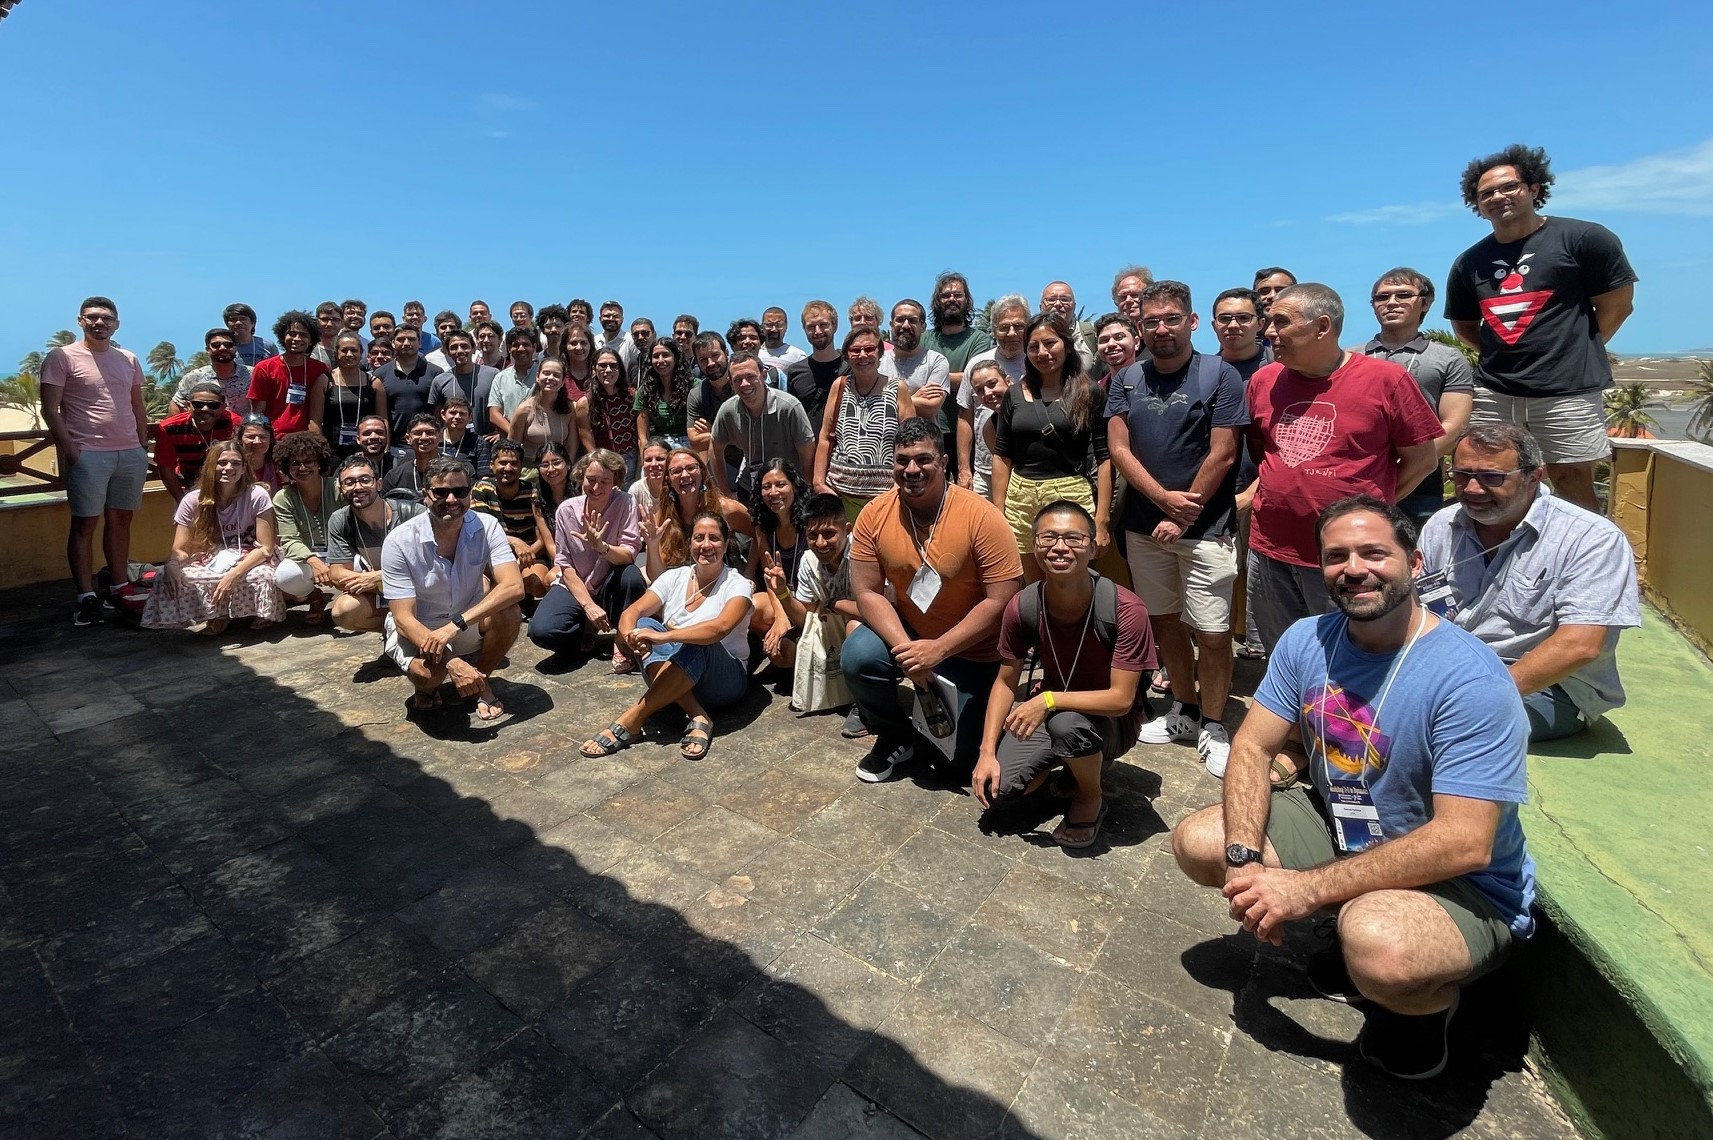
\includegraphics[width=8.5cm]{Workshop2.jpg}
    \caption{Participantes no Workshop 2+3 in Dynamics.}
 \label{workshop2}
\end{figure}


O comitê organizador foi formado por Aline Melo (UFC), Cristina Lizana (UFBA), Elaís Malheiro (UFBA), Edgar Matias (UFBA), Mauricio Poletti (UFC), Roberto Sant'Anna (UFBA) e Yuri Lima (UFC). O evento contou com a participação de pesquisadores de diversas instituições do Nordeste, do Brasil e de diversos países, promovendo a integração e o intercâmbio de conhecimentos entre os cerca de 80 participantes.


O Workshop 2+3 in Dynamics evidenciou a diversidade da Teoria de Sistemas Dinâmicos, com palestras que exploraram desde formalismo termodinâmico, com foco em operadores de transferência e medidas invariantes em certos espaços, até dinâmica hiperbólica, com a investigação sobre condições para garantir existência de hiperbolicidade em certos sistemas dinâmicos.  Sistemas parcialmente hiperbólicos e teoria ergódica também foram temas de destaque, com estudos sobre  difeomorfismos e  aplicações em  bilhares caóticos.

 O evento contou com 16 plenárias de pesquisadores internacionais, sendo 6 delas ministradas por mulheres. Além das palestras, o evento contou com três sessões de apresentação de pôsteres e momentos de discussão, incentivando o intercâmbio de ideias e a colaboração entre os presentes. Gostariamos de dar destaque à delegação da UFBA, formada por docentes e discentes de graduação, mestrado e doutorado (Fig. \ref{workshop1}).


%Incluir outra imagem aqui (possivelmente com interação entre os participantes)
\begin{figure}[htb]
    \centering
    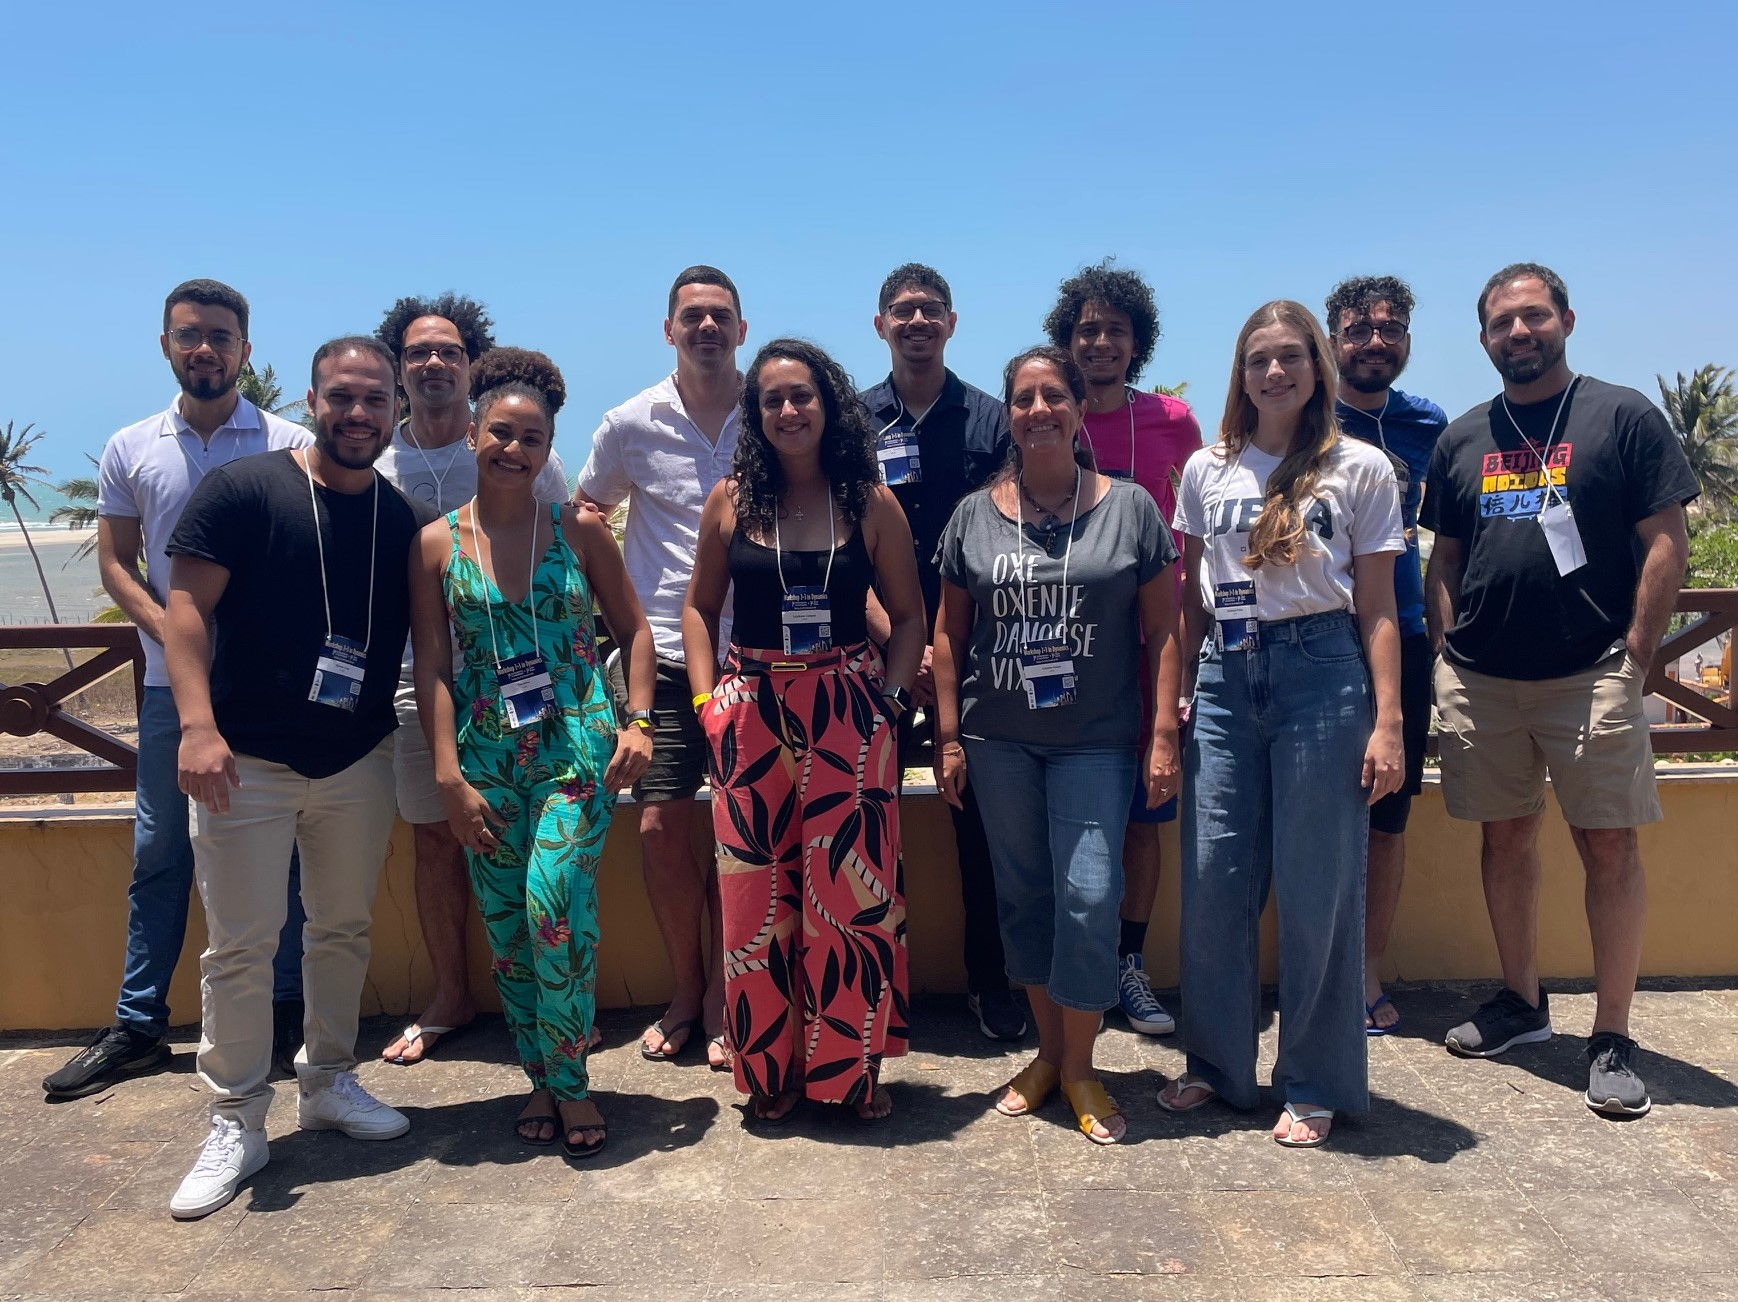
\includegraphics[width=8.5cm]{Workshop1.jpg}
    \caption{Delegação da UFBA no Workshop 2+3 in Dynamics.}
 \label{workshop1}
\end{figure}


Além do aprofundamento teórico, o evento estimulou a colaboração entre pesquisadores, abrindo caminhos para novas parcerias e projetos de pesquisa.  O Workshop 2+3 in Dynamics consolidou-se como um importante fórum para o desenvolvimento e a disseminação da pesquisa em Sistemas Dinâmicos no Nordeste do Brasil, contribuindo significativamente para o avanço da área no país.


Para mais informações sobre o Workshop 2+3 in Dynamics, acesse o site
\href{https://sites.google.com/view/workshop23indynamics}{https://sites.google.com/view/workshop23indynamics}.


\section{3\superou Encontro Brasileiro de Mulheres Matemáticas }

De 13 a 16 de novembro de 2024, a Universidade Federal da Bahia teve o privilégio de sediar o ``3\superou Encontro Brasileiro de Mulheres Matemáticas'' (3\superou EBMM), evento que teve coordenação da Prof.\superau Simone Moraes, do Departamento de Matemática da UFBA.
O evento teve as edições anteriores realizadas no Rio de Janeiro em 2019 e em Belém do Pará em 2022, consolidando-se como um espaço para discussão sobre a questão de gênero na Matemática, bem como de divulgação e promoção da Matemática desenvolvida por mulheres no Brasil.

Com o objetivo de fortalecer a integração, promover discussões sobre inclusão e destacar o papel das mulheres na Matemática em todo o Brasil, o evento mostrou o seu alcance nacional já na organização, com comissão organizadora integrada por Simone Maria de Moraes (UFBA), Barbara Corominas Valério (USP), Elaís Cidely Souza Malheiro (UFBA), Elen Deise Assis Barbosa (UFBA), Janice Pereira Lopes (UFG), Juliana Silva Canella (UFPA), Juliana Ferreira Ribeiro de Miranda (UFAM), Manuela da Silva Souza (UFBA) e Sylvia Ferreira da Silva (UFRPE) e comitê científico composto por Adriana Neumann de Oliveira (UFRGS), Alice de Jesus Kozakevicius (UFSM), Ana Paula de Araújo Chaves (UFG), Cláudia Aline Azevedo dos Santos Mesquita (UNIFESP), Juliana Fernandes da Silva Pimentel (UFRJ), Kátia Maria de Medeiros (UEPB), Kelly Karina Santos (UFRR), Manuela da Silva Souza (UFBA), Simone de Almeida Delphim Leal (UNIFAP) e Vanessa Franco Neto (UFMS).

\begin{figure}[htb]
    \centering
    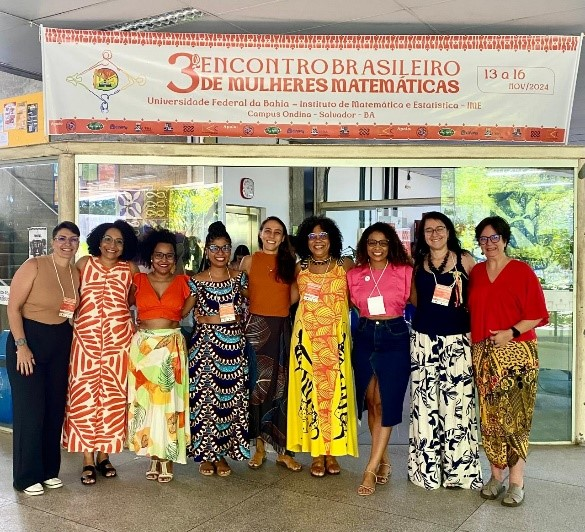
\includegraphics[width=8.5cm]{EBMM3.jpg}
    \caption{Comissão Organizadora do 3\superou EBMM.}
 \label{EBMM3}
\end{figure}

Nesta edição o evento teve uma abrangência expressiva, contando com quase 250 participantes, vindas de todas as regiões do Brasil e a organização preparou uma programação ampla e diversa, proporcionando momentos para uma intensa interação entre estudantes, jovens pesquisadoras e matemáticas experientes. O evento foi um espaço para a divulgação de pesquisas científicas, projetos inovadores e iniciativas transformadoras, além das trocas significativas de conhecimentos e vivências.

\begin{figure}[htb]
    \centering
    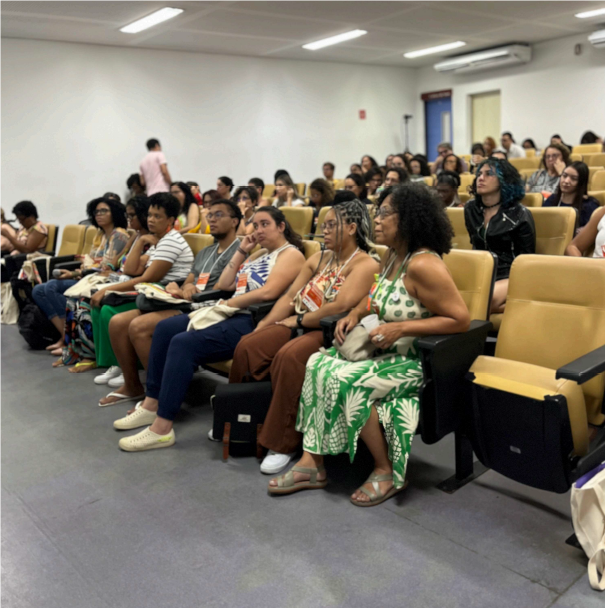
\includegraphics[width=8.5cm]{EBMM4.png}
    \caption{Participantes no auditório do IME.}
 \label{EBMM4}
\end{figure}

A programação incluiu quatro palestras de pesquisadoras de destaque no cenário nacional e internacional e seis palestras curtas apresentadas por jovens pesquisadoras, que trouxeram temas relevantes e atuais da Matemática em geral. Além disso, o evento contou com quatro sessões de pôsteres, que reuniram cerca de 90 trabalhos das áreas de Educação e Ensino de Matemática, Matemática e Matemática Aplicada, e Gênero.

Um destaque significativo do 3\superou EBMM foram as três mesas de discussão, que abordaram temas centrais sobre desigualdades de gênero e étnico-racial na academia, equidade e inclusão na comunidade Matemática brasileira e desafios e conquistas de mulheres em suas trajetórias na Matemática. Também se destacaram as duas sessões de ``Projetos de Inclusão, de Divulgação e de Outras Iniciativas'', nas quais foram apresentados projetos voltados a motivar e fortalecer a presença de meninas e jovens mulheres na Matemática e ciências exatas. Além disso, vídeos curtos com relatos de vivências de mulheres na Matemática enriqueceram as reflexões ao longo do evento.

\begin{figure}[htb]
    \centering
    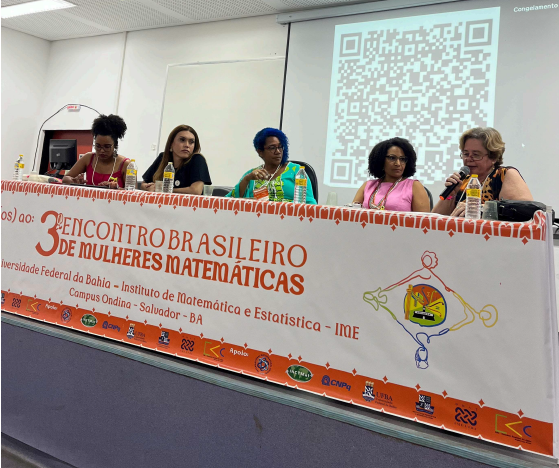
\includegraphics[width=8.5cm]{EBMM1.png}
    \caption{Registro de uma das mesas de discussão.}
 \label{EBMM1}
\end{figure}

Programação à parte, dois destaques no evento foram: a participação expressiva de estudantes da UFBA foi um ponto a se comemorar, muitas(os) se incorporaram à organização local imprimindo um pouco de baianidade nos detalhes, desde a recepção, com os materiais de credenciamento, até os momentos de intervalos e de confraternização e, não menos importante, foi o primeiro encontro presencial das mulheres do coletivo ``Matemáticas Negras'', no 3\superou EBMM.

\begin{figure}[htb]
    \centering
    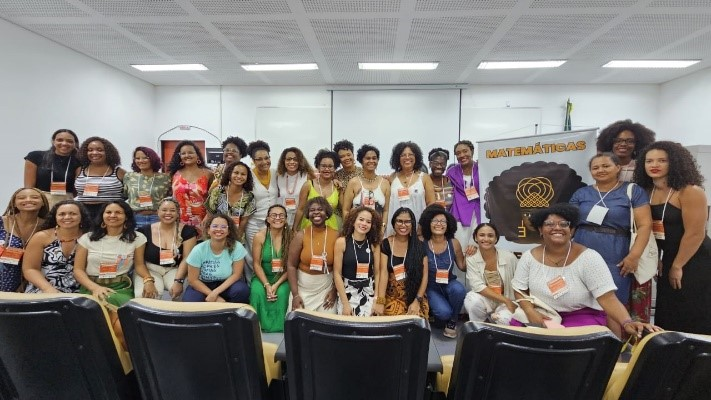
\includegraphics[width=8.5cm]{EBMM2.jpg}
    \caption{Registro de encontros das participantes.}
 \label{EBMM2}
\end{figure}

Assim, mantendo a filosofia das edições anteriores, o encontro logrou reunir mulheres de diversas áreas da Matemática, desde estudantes do ensino médio até pesquisadoras experientes, consolidando-se ainda mais como um espaço de fortalecimento, empoderamento e união, mostrando o brilho, a força e o impacto das mulheres na Matemática e reafirmando seu papel transformador no cenário acadêmico e científico do Brasil.

O 3\superou EBMM foi um sucesso, com vários momentos emocionantes, muitos abraços e sobretudo celebração das mulheres na matemática. Finalizou deixando um gostinho de saudade.

Que venha a quarta edição!

%Após o  sucesso das duas primeiras edições do Encontro Brasileiro de Mulheres na Matemática (EBMM), realizadas no Rio de Janeiro e no Pará, a Universidade Federal da Bahia teve o privilégio de sediar o 3° EBMM, que ocorreu em novembro de 2024 sob a coordenação da Prof.\superau Simone Moraes, do Departamento de Matemática da UFBA.

 

 %Com o objetivo de fortalecer a integração, promover discussões sobre inclusão e destacar o papel das mulheres na Matemática em todo o Brasil, o evento mostrou o seu alcance nacional já na composição das comissões organizadora e científica, que foram compostas pelas professoras:  Adriana Neumann de Oliveira (UFRGS), Alice de Jesus Kozakevicius (UFSM), Ana Paula de Araújo Chaves (UFG), Barbara Corominas Valerio (USP),  Cláudia Aline Azevedo dos Santos Mesquita (UNIFESP), Elaís Cidely Souza Malheiro (UFBA), Elen Deise Assis Barbosa (UFBA), Janice Pereira Lopes (UFG),   Juliana Fernandes da Silva Pimentel (UFRJ), Juliana Silva Canella (UFPA), Juliana Ferreira Ribeiro de Miranda (UFAM), Kátia Maria de Medeiros (UEPB), Kelly Karina Santos (UFRR), Manuela da Silva Souza (UFBA), Sylvia Ferreira da Silva (UFRPE),  Simone de Almeida Delphim Leal (UNIFAP), Simone Moraes(UFBA) e Vanessa Franco Neto (UFMS).

 

%Com quase 200 participantes inscritas de todas as regiões do Brasil, o 3\superou EBMM ofereceu uma rica programação entre os dias 13 e 16 de novembro, promovendo intensa interação entre pesquisadoras jovens e experientes. O evento foi um espaço para a divulgação de pesquisas científicas, projetos inovadores e iniciativas transformadoras, além de oportunizar trocas significativas de conhecimentos e vivências.

 

%A programação incluiu quatro palestras de pesquisadoras de destaque no cenário nacional e internacional e seis palestras curtas apresentadas por jovens pesquisadoras, que trouxeram temas relevantes e atuais da Matemática. Além disso, o evento contou com quatro sessões de pôsteres, que reuniram cerca de 70 trabalhos das áreas de Educação e Ensino de Matemática, Matemática e Matemática Aplicada, e  Gênero.

 

%Um destaque significativo do 3\superou EBMM foram as três mesas de discussão, que abordaram temas centrais sobre inclusão, equidade e desafios das mulheres na matemática. Também se destacaram as duas sessões  de Projetos de Inclusão, de Divulgação e de Outras Iniciativas, nas quais foram apresentados projetos voltados a motivar e fortalecer a presença de meninas e jovens mulheres na Matemática e ciências exatas. Além disso, vídeos curtos com relatos de vivências de mulheres na Matemática enriqueceram as reflexões ao longo do evento.

 

%Mantendo o legado das edições anteriores, a terceira edição do EBMM foi um sucesso! Se consolidou ainda mais como um espaço de celebração, empoderamento e avanço, mostrando o brilho, a força e o impacto das mulheres na Matemática e reafirmando seu papel transformador no cenário acadêmico e científico do Brasil.



\section{IX Encontro da Pós-graduação em Matemática da UFBA} % (Cris) %~(Henrique)
%Entre os dias 18 e 22 de novembro de 2024, foi realizado o IX Encontro da Pós-graduação em Matemática da UFBA (EPGMAT) no Auditório Maria José ``Zezé'' de Oliveira no IME-UFBA (Fig. \ref{epgmat}). 
%
%\begin{figure}[htb]
%    \centering
%    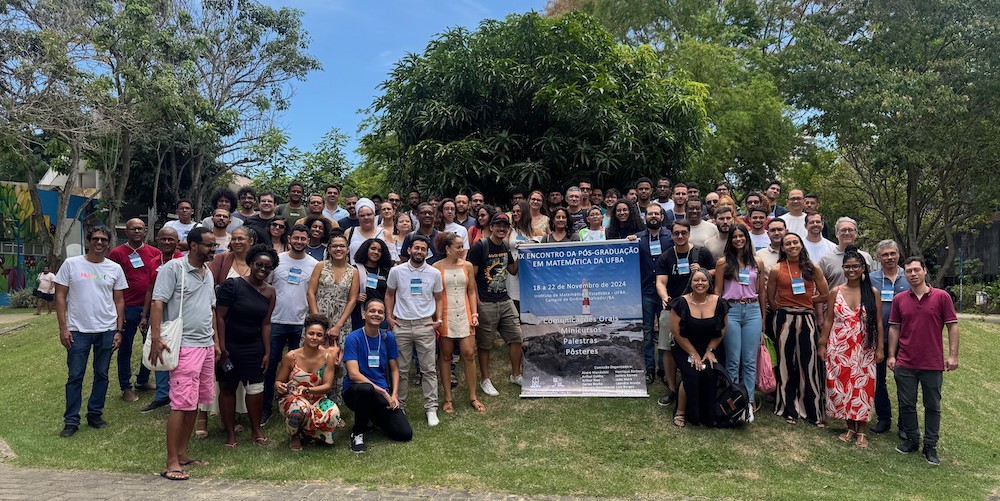
\includegraphics[width=8.5cm]{9epgmat.jpg}
%    \caption{IX Encontro da Pós-graduação em Matemática da UFBA.}
% \label{epgmat}
%\end{figure}
%
%O encontro acontece anualmente no segundo semestre de cada ano letivo, dirigido a docentes, pesquisadores e alunos de cursos de Mestrado e Doutorado em Matemática e Estatística, tanto da UFBA como de outras instituições de ensino superior no Brasil. Também estão aptos a participar os alunos de cursos de graduação. Palestras e minicursos são ministrados por docentes do Programa de Pós-Graduação em Matemática da UFBA e do Programa de Doutorado em Matemática UFBA/UFAL e convidados. 
%
%O objetivo principal do encontro é divulgar os trabalhos do corpo docente e discente dos dois programas e promover a interação entre os participantes, enriquecendo o ambiente de trabalho de ensino e pesquisa, contribuindo para a difusão da Matemática, Estatística e áreas afins.
%
%Para mais informações sobre o Encontro da Pós-graduação em Matemática da UFBA, acesse \href{https://encontropgmat.ufba.br/}{https://encontropgmat.ufba.br/}.

Entre os dias 18 e 22 de novembro de 2024, foi realizado o IX Encontro da Pós-graduação em Matemática da UFBA (EPGMAT) no Instituto de Matemática e Estatística (IME) da UFBA (Fig. \ref{epgmat}). O EPGMAT foi uma experiência transformadora, marcada por aprendizado, troca de ideias e conexões significativas. 

\begin{figure}[htb]
    \centering
    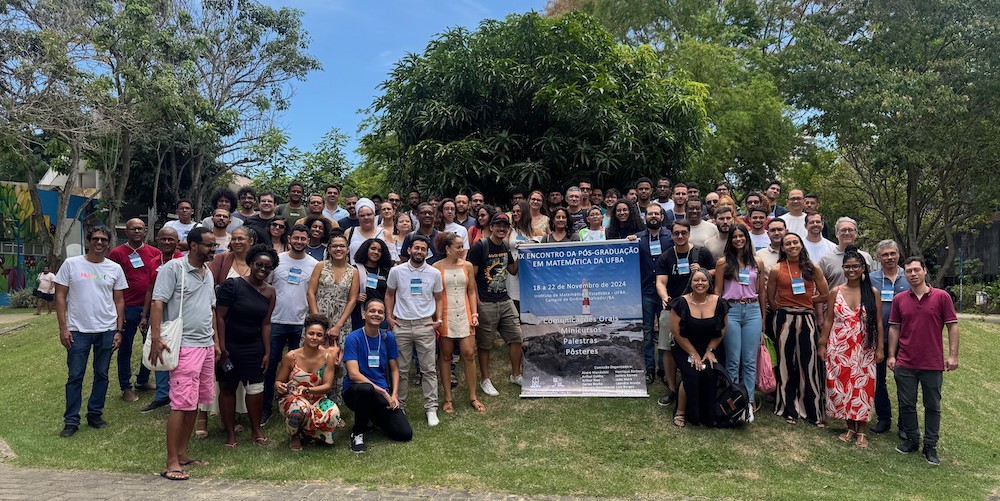
\includegraphics[width=8.5cm]{9epgmat.jpg}
    \caption{IX Encontro da Pós-graduação em Matemática da UFBA.}
 \label{epgmat}
\end{figure}

O evento contou com palestras ministradas por professores do Programa de Pós-Graduação em Matemática da UFBA e também por convidados externos, que abordaram temas de pesquisa de ponta, inspirando os participantes a expandirem seus horizontes acadêmicos. As comunicações orais e as sessões de pôsteres também desempenharam um papel central, oferecendo um espaço dinâmico para a divulgação de pesquisas, a troca de ideias e a construção de parcerias colaborativas. Entre as atividades, destacaram-se ainda três minicursos oferecidos, com especial ênfase para ``Python para Matemáticos'', explorando novas aplicações tecnológicas no campo da Matemática e Estatística. 



O encontro acontece no segundo semestre de cada ano letivo, é organizado e dirigido a docentes, pesquisadores e alunos dos cursos de pós-graduação de programas de Matemática e Estatística, tanto da UFBA como de outras instituições de ensino superior no Brasil. 
No entanto, alunos de cursos de graduação também são bem vindos e são incentivados a participar do encontro.


Os principais objetivos do encontro são a divulgação e aprofundamento do conhecimento em Matemática e Estatística e o fomento à interação entre alunos e professores, participantes e convidados, buscando a integração entre a comunidade acadêmica dos programas de pós-graduação do IME com a comunidade externa à UFBA, contribuindo para a difusão da Matemática, Estatística e áreas afins.

Na IX edição foram apresentadas 14 palestras, 3 minicursos, 1 mesa redonda, 17 comunicações orais de discentes do doutorado e 30 pôsteres de discentes da graduação e do mestrado.
Uma das principais novidades desta edição foi a participação do Mestrado Profissional em Matemática em Rede Nacional (PROFMAT), que integrou o encontro pela primeira vez, trazendo perspectivas enriquecedoras e fomentando a interação entre diferentes públicos. 
%
%Mais ainda, esta foi a primeira edição a contar com a participação de alunos e professores do Mestrado Profissional em Matemática em Rede Nacional (PROFMAT) da UFBA.

Mais do que um encontro científico, o IX EPGMAT reafirmou seu papel como um espaço de crescimento, colaboração e valorização da matemática em suas diversas dimensões.

Para mais informações sobre o Encontro da Pós-graduação em Matemática da UFBA, acesse \href{https://encontropgmat.ufba.br/}{https://encontropgmat.ufba.br}.

%%%%%%%%%%%%%%%%%%%%%%%%%%%%%%%%%%%%%%%%%%%%%%%%%%%%%%%%%%%%%%%%%%%%%%%%%%%%%%%%%%%%%%%
%\vspace{.5cm} 
%\textbf{Enviado pelo Arthur}
%O *IX Encontro da Pós-Graduação em Matemática da UFBA (EPGMAT)*, realizado de 18 a 22 de novembro de 2024, 
%
%foi uma experiência transformadora, marcada por aprendizado, troca de ideias e conexões significativas. O evento contou com palestras ministradas por professores do programa e convidados externos, que abordaram temas de pesquisa de ponta, inspirando os participantes a expandirem seus horizontes acadêmicos. As comunicações orais e as sessões de pôsteres também desempenharam um papel central, oferecendo um espaço dinâmico para a divulgação de pesquisas, a troca de ideias e a construção de parcerias colaborativas. Entre as atividades, destacaram-se ainda três minicursos oferecidos, com especial ênfase para *Python para Matemáticos*, explorando novas aplicações tecnológicas no campo da matemática/estatística. 

%Uma das principais novidades desta edição foi a participação do *Mestrado Profissional em Matemática em Rede Nacional (PROFMAT)*, que integrou o encontro pela primeira vez, trazendo perspectivas enriquecedoras e fomentando a interação entre diferentes públicos. 
%
%O IX EPGMAT destacou-se como um evento essencial para promover o sentimento de pertencimento e fortalecer os laços entre estudantes, professores e pesquisadores. O encerramento, com uma confraternização calorosa, celebrou o sucesso do evento e a integração da comunidade acadêmica.  
%
%Mais do que um encontro científico, o IX EPGMAT reafirmou seu papel como um espaço de crescimento, colaboração e valorização da matemática em suas diversas dimensões.


% \section{Olimpiadas} %8a OMEBA e cerimônia de premiação} %Henrique

% As Olimpíadas de Matemática estão estabelecidas na cultura escolar do Brasil. 
%        A OBMEP  está desde 2005 fomentando a discussão científica e a descoberta de novos talentos, aumentando a cada ano o número de escolas e alunos participantes.
%        
%        Já a Olimpíada Brasileira de Matemática (OBM), realizada pela Associação Olimpíada Brasileira de Matemática (AOBM), com apoio da UFBA, e voltada para alunos desde o 6\superou ano do Ensino Fundamental até o Ensino Médio, é a principal porta de entrada para competições internacionais.
%        Uma das maneiras de participar da OBM é por meio das olimpíadas estaduais, em que a Olimpíada de Matemática do Estado da Bahia (OMEBA) apresenta sua cara.
%        
%        Desde 2013, a OMEBA é realizada em uma parceria do DMAT e da AOBM.
%        Devido à pandemia de COVID-19 as provas da OMEBA foram realizadas de forma virtual.
%        A edição de 2024 marcou a volta de provas presenciais e contou com a presença de pelo menos 600 estudantes, em diversos polos de aplicação, na cidade de Salvador e no interior do estado.
%%        
%%         \begin{figure}[htb]
%%    \centering
%%    \includegraphics[width=8cm]{omeba1.jpg}
%%    \caption{Público presente na cerimônia de premiação da OMEBA em 30 de novembro de 2023.}
%% \label{omeba1}
%%\end{figure}
%
%        
%        Como em toda competição, os melhores participantes são premiados com medalhas e a Cerimônia de Premiação da OMEBA ocorreu no dia 30 de Novembro de 2023 no Salão Nobre da Reitoria da UFBA, em Salvador (Fig. \ref{omeba1}).        A ilustre cerimônia ocorreu com a presença dos professores Kleyber Mota da Cunha, representando o IME-UFBA; Darllan Conceição Pinto, representando o DMAT; Evandro Carlos Ferreira dos Santos, na ocasião representando a OMEBA; além da professora Vanessa Balbina da Silva Lopes Miguel, da Escola SESI Djalma Pessoa, e o professor Antônio Márcio de Lima Soares, do Instituto Federal da Bahia (IFBA) representando os professores das escolas participantes (Fig. \ref{omeba2}).
%        Quase uma centena de alunos e alunas foram homenageados com medalhas de bronze, prata e ouro, devido ao seu desempenho nos três níveis de competição.
%               
%%         \begin{figure}[htb]
%%    \centering
%%    \includegraphics[width=8cm]{omeba2.jpg}
%%    \caption{Professores presidindo a cerimônia.}
%% \label{omeba2}
%%\end{figure}
%
%     Para mais informações da OMEBA, acesse \href{https://www.omeba.ufba.br}{https://www.omeba.ufba.br}.
% 
%        
%

%\section{Aulão Olímpico: Superando Desafios em Matemática}

%Alguma imagem representativa do Aulão

%O IME-UFBA abriu suas portas para 85 estudantes de escolas públicas de Salvador e Camaçari, em um dia dedicado à descoberta e ao aprofundamento da matemática. O "Aulão Olímpico: Superando Desafios em Matemática", um projeto de extensão do DMAT-UFBA, visa fortalecer a cultura de Matemática Olímpica na região, proporcionando uma experiência enriquecedora e inspiradora para jovens apaixonados por desafios.  

%O projeto busca  despertar o interesse dos estudantes pelas competições de matemática, como a OBMEP, e  incentivá-los a trilhar caminhos acadêmicos, por meio de encontros realizados ao longo do ano letivo. Na ocasião do último dia 17 de outubro, através de aulas desafiadoras em diferentes níveis, os alunos exploraram o universo das Olimpíadas de Matemática e aprimoraram suas habilidades. A psicóloga Taíris Araújo conduziu uma sessão especial sobre gestão emocional para provas, auxiliando os estudantes a lidarem com a ansiedade e a alcançarem seu máximo potencial.

%Imagem da atuação da psicóloga.

%A visita ao Planetário da UFBA complementou a experiência, mostrando a conexão da matemática com outras áreas do conhecimento e despertando a curiosidade dos participantes. O Aulão Olímpico busca não apenas fortalecer as habilidades matemáticas dos estudantes, mas também inspirá-los a vislumbrar a universidade como um espaço acessível e possível. Com potencial de expansão futuro para outros municípios, o projeto  reuniu estudantes, professores e colaboradores em um ambiente de aprendizado, colaboração e paixão pela matemática,  impactando positivamente a comunidade e abrindo portas para novas oportunidades.

%Imagem da visita ao Planetário.

%Vale salientar que o Aulão Olímpico teve um impacto significativo na vida dos participantes. O feedback dos estudantes e professores foi extremamente positivo, demonstrando o entusiasmo e a satisfação com a iniciativa. Para muitos estudantes, essa foi a primeira oportunidade de vivenciar o ambiente universitário, despertando o sonho de ingressar na UFBA e seguir carreira acadêmica. O projeto  "Aulão Olímpico: Superando Desafios em Matemática"  cumpriu seu papel de inspirar e transformar, mostrando aos jovens o poder da educação e abrindo portas para um futuro promissor.

%Para mais informações sobre tudo o que acontece no mundo das Olimpíadas de Matemática em Salvador e Região Metropolitana, visitem o perfil do projeto Matemática Olímpica no Instagram!

%\href{https://www.instagram.com/mat.olimpica/#}{@mat.olimpica}



\section{Olimpíadas de Matemática: um ano de conquistas e desafios}

As Olimpíadas de Matemática estão estabelecidas na cultura escolar do Brasil. A OBMEP, desde 2005, fomenta a discussão científica e a descoberta de novos talentos, aumentando a cada ano o número de escolas e alunos participantes. Já a Olimpíada Brasileira de Matemática (OBM), realizada pela Associação Olimpíada Brasileira de Matemática (AOBM), com apoio da UFBA, e voltada para alunos desde o 6\superou ano do Ensino Fundamental até o Ensino Médio, é a principal porta de entrada para competições internacionais. Outra competição que se faz presente no âmbito estadual é a Olimpíada de Matemática do Estado da Bahia (OMEBA), coordenada pelos professores do DMAT Henrique Barbosa, Roberto Sant'Anna e Samuel Feitosa. Vale ressaltar que essa competição está habilitada para ser uma das maneiras de participar da OBM.

O Departamento de Matemática %da UFBA (DMAT)
e o Instituto de Matemática e Estatística da UFBA %(IME)
têm sido protagonistas nesse cenário, organizando e apoiando diversos eventos relacionados às Olimpíadas de Matemática. Acreditamos que essas iniciativas são fundamentais para a formação dos estudantes, incentivando o desenvolvimento do raciocínio lógico, a criatividade e o gosto pela Matemática. As Olimpíadas de Matemática promovem a inclusão social, despertam a curiosidade científica e revelam jovens talentos, tanto em nível nacional quanto local.

Em Salvador e Região Metropolitana, o DMAT e o IME têm concentrado esforços para o crescimento e desenvolvimento das Olimpíadas de Matemática, apoiando projetos como a OBM, OBMEP, OMEBA e OFMEBA, entre outras iniciativas, e também organizando e realizando eventos como cerimônias de premiação, aulões e visitas em diversos setores da sociedade ligados à educação, tendo em vistas contribuir com os mesmo de forma positiva. A seguir, apresentamos os destaques do período.

\vspace{0.5cm}

{\bf \noindent Cerimônia de Premiação da OBMEP}

\vspace{0.5cm}

A Olimpíada Brasileira de Matemática das Escolas Públicas (OBMEP) é um projeto de grande relevância nacional, despertando o interesse e o entusiasmo pela matemática em estudantes de escolas públicas de todo o país. O DMAT tem um papel fundamental na organização da OBMEP em nível local, atuando na aplicação das provas e na realização da Cerimônia de Premiação Regional.

\begin{figure}[htb]
    \centering
    \includegraphics[width=8.5cm]{olimp1.jpg}
    \caption{Alunos e convidados para a Cerimônia de Premiação da OBMEP.}
 \label{olimp1}
\end{figure}

No dia 17 de junho de 2024, o Salão Nobre da Reitoria da UFBA foi palco da Cerimônia de Premiação da OBMEP, reunindo cerca de 150 pessoas, entre alunos medalhistas de ouro, prata e bronze de Salvador e Região Metropolitana, seus familiares, professores e convidados. O evento celebrou o talento e a dedicação desses jovens, reconhecendo seus esforços e incentivando a busca por novos desafios.



A cerimônia contou com a presença do Reitor da UFBA, Paulo Cesar Miguez de Oliveira, e do Diretor do IME, Kleyber Mota, além de outras autoridades e representantes da comunidade acadêmica. A mesa foi composta por Roberto Sant'Anna, Coordenador Regional da OBMEP; Rosilene Cavalcante, Superintendente de Políticas Públicas para a Educação Básica da SEC-BA; Isnard Araújo, vereador da cidade de Salvador; Isabela Cavalcanti, representante da SMED-Salvador; e Patrícia Ribeiro, Coordenadora Pedagógica do NTE 26.

\begin{figure}[htb]
    \centering
    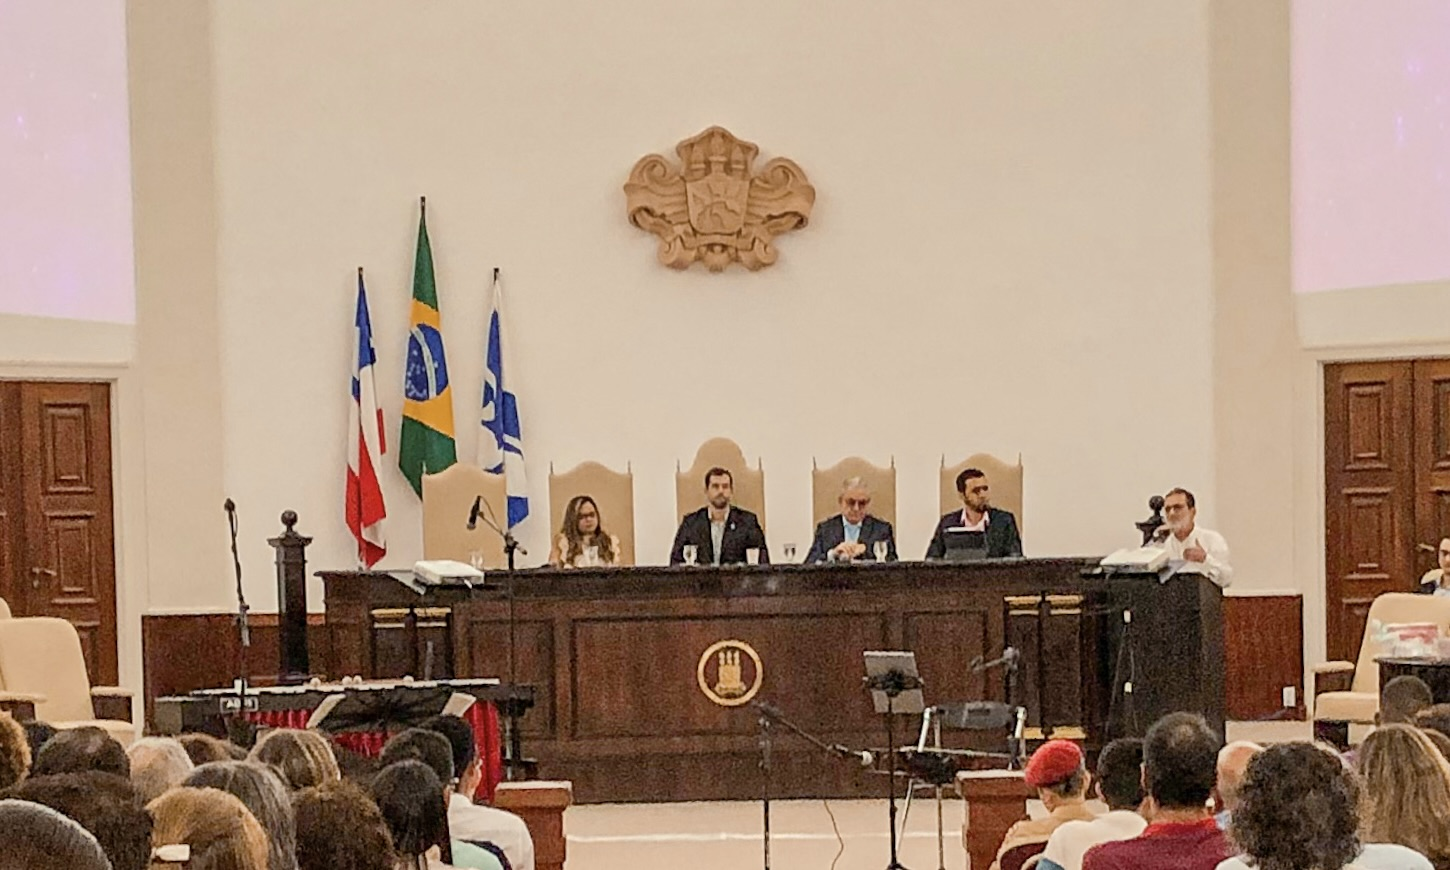
\includegraphics[width=8.5cm]{olimp2.jpeg}
    \caption{Mesa principal da Cerimônia, contando com a presença do Reitor da UFBA, Paulo Cesar Miguez de Oliveira.}
 \label{olimp2}
\end{figure}

O Duo VibraCor, formado pelos professores da UFBA Ricardo Camponogara e Aquim Sacramento, abrilhantou a cerimônia com belas canções, emocionando a todos os presentes.

%\begin{figure}[htb]
%    \centering
%     \includegraphics[width=8.5cm]{olimp3.jpg}
%     \caption{IX Encontro da Pós-graduação em Matemática da UFBA.}
% \label{olimp3}
%\end{figure}

\vspace{0.5cm}

{\bf \noindent Aulão Olímpico: Superando Desafios em Matemática}

\vspace{0.5cm}

O projeto de extensão ``Aulão Olímpico: Superando Desafios em Matemática'', do DMAT, visa fortalecer a cultura de Matemática Olímpica na região, proporcionando uma experiência enriquecedora para jovens apaixonados por desafios. No dia 17 de outubro de 2024, o IME abriu suas portas para 85 estudantes de escolas públicas de Salvador e Camaçari, em um dia dedicado à descoberta e ao aprofundamento da matemática.

\begin{figure}[htb]
    \centering
    \includegraphics[width=8.5cm]{olimp4.jpg}
    \caption{Momento da fala acolhedora da psicóloga Taíris Araújo com os estudantes.}
 \label{olimp4}
\end{figure}

Os alunos participaram de aulas desafiadoras em diferentes níveis, explorando o universo das Olimpíadas de Matemática e aprimorando suas habilidades. A psicóloga Taíris Araújo conduziu uma sessão especial sobre gestão emocional para provas, auxiliando os estudantes a lidarem com a ansiedade e a alcançarem seu máximo potencial. A visita ao Planetário da UFBA complementou a experiência, despertando a curiosidade e mostrando a conexão da matemática com outras áreas do conhecimento.

\begin{figure}[htb]
    \centering
    \includegraphics[width=8.5cm]{olimp5.jpg}
    \caption{Visita dos estudantes do Aulão ao Planetário da UFBA.}
 \label{olimp5}
\end{figure}

O Aulão Olímpico busca não apenas fortalecer as habilidades matemáticas dos estudantes, mas também inspirá-los a vislumbrar a universidade como um espaço acessível e possível. O projeto reuniu estudantes, professores e colaboradores em um ambiente de aprendizado, colaboração e paixão pela matemática, impactando positivamente a comunidade e abrindo portas para novas oportunidades.

\vspace{0.5cm}

{\bf \noindent OMEBA, OFMEBA e outras iniciativas}

\vspace{0.5cm}

A Olimpíada de Matemática do Estado da Bahia (OMEBA) e a Olimpíada Feminina de Matemática do Estado da Bahia (OFMEBA) também foram destaques no ano de 2024. As provas da OMEBA, realizadas em 25 de agosto de 2024, contaram com a participação de 600 estudantes em diversos polos de aplicação na Bahia.

A cerimônia de premiação da OFMEBA, realizada em 10 de setembro de 2024, foi recheada de momentos de grande emoção para as medalhistas, que celebraram suas conquistas ao lado de professores, familiares e autoridades. O DMAT atuou como parceiro na organização desse evento, que é coordenado pelo professor Acélio Rodrigues (IFBA), contribuindo para o sucesso das Olimpíadas. A OFMEBA, em especial, tem um papel fundamental no incentivo à participação feminina na matemática, mostrando que as meninas também podem se destacar nessa área.

O DMAT também esteve presente em outras iniciativas relacionadas às Olimpíadas de Matemática. Em 25 de setembro de 2024, participamos como parceiros da Cerimônia de Premiação Regional da Secretaria Municipal de Educação de Salvador (SMED), celebrando o talento e a dedicação dos estudantes premiados.

%\vspace{0.5cm}

{\bf \noindent E para o futuro?}

%\vspace{0.5cm}

Para as próximas edições das Olimpíadas de Matemática, esperamos ampliar o alcance das atividades, aumentar a participação dos estudantes e promover novas iniciativas que contribuam para o desenvolvimento da educação matemática na Bahia.

Para mais informações sobre as Olimpíadas de Matemática em Salvador e Região Metropolitana, visitem o perfil do projeto Matemática Olímpica no Instagram: \href{https://www.instagram.com/mat.olimpica/#}{@mat.olimpica}.



%%%%%%%%%%%%%%%%%%
%%%%%%%%Bio
\vspace{1.5cm}
%\vfill\eject
\begin{wrapfigure}{L}{1.7cm}
	\vspace{-10pt}
	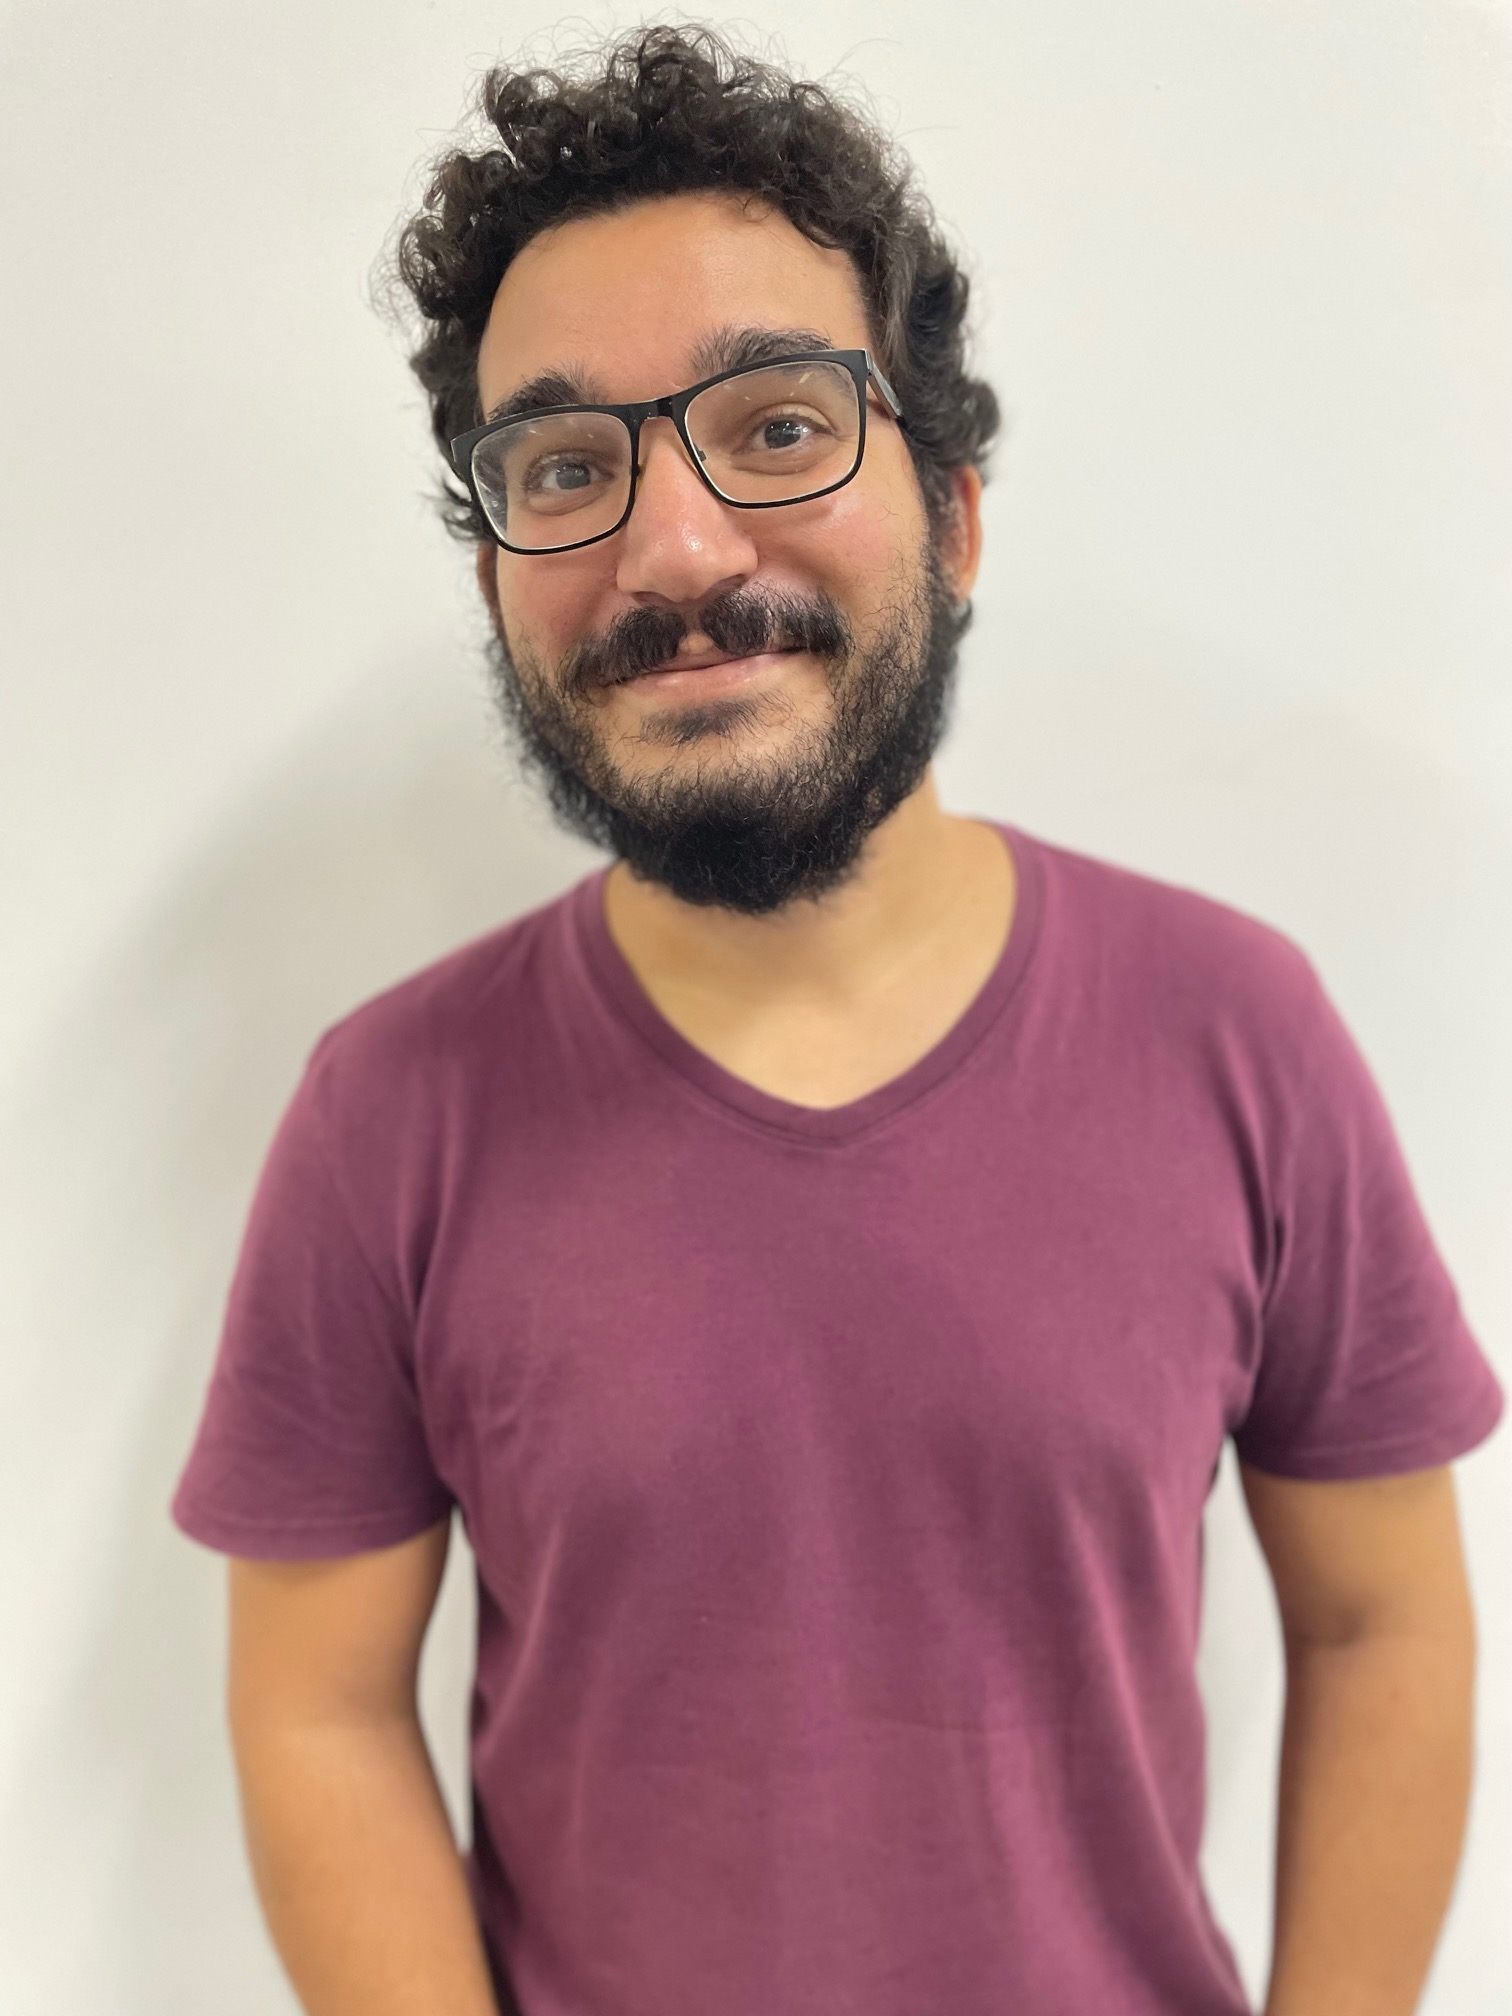
\includegraphics[width=2cm]{Henrique.jpg}
\end{wrapfigure}\noindent  
  Henrique da Costa é mineiro, cursou graduação e pós-graduação 
  no ICMC-USP em São Carlos, interior de São Paulo, e está na UFBA em Salvador 
  desde 2016. Atua na área de pesquisa em análise, mais precisamente sistemas 
  dinâmicos não-lineares e equações diferenciais parciais. 
  Estuda piano e jogos de cartas e tabuleiro como hobby. 
  Foi cabeludo durante a pandemia, no entanto não se atreveu a ser padeiro.
\vspace{0.5cm}
\pagebreak 

\begin{wrapfigure}{L}{1.7cm}
	\vspace{-0pt}
	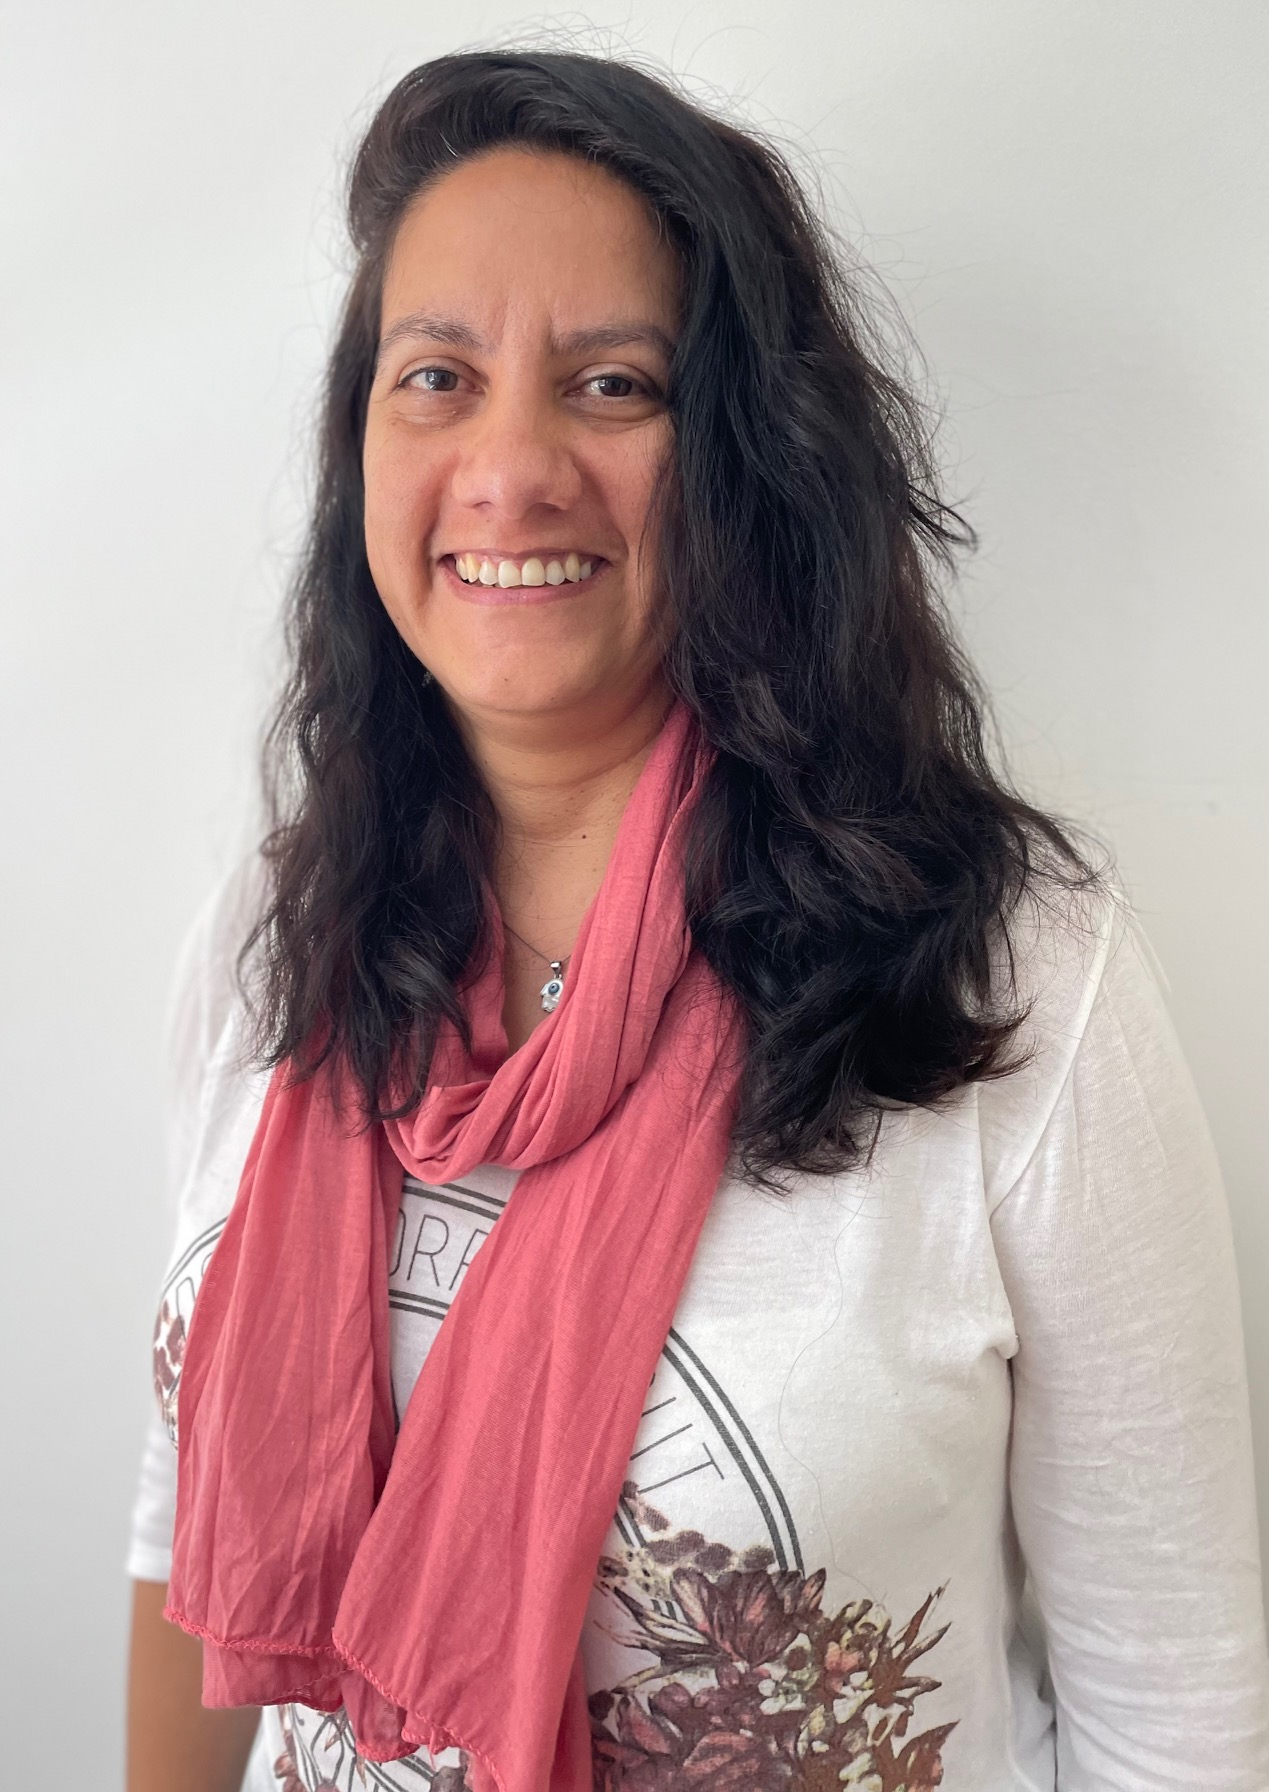
\includegraphics[width=2cm]{Cristina.jpg}
\end{wrapfigure}\noindent  
Cristina Lizana é venezuelana, com graduação e mestrado em Matemática 
pela Universidad de Los Andes-ULA (Venezuela), e doutorado em Matemática pelo IMPA (Brasil).
Foi professora da ULA (2004-2017) e trabalha na UFBA desde 2018. Pesquisa na área de 
Sistemas Dinâmicos, atuando principalmente em Dinâmica Parcialmente Hiperbólica 
e mapas robustamente transitivos. Atualmente, é a coordenadora do Núcleo de Extensão do IME e vice-coordenadora do Mestrado em Matemática. O seu hobby é a fotografia e a estreita relação desta com a matemática.

\vspace{0.5cm}
\begin{wrapfigure}{L}{1.7cm}
	\vspace{-10pt}
	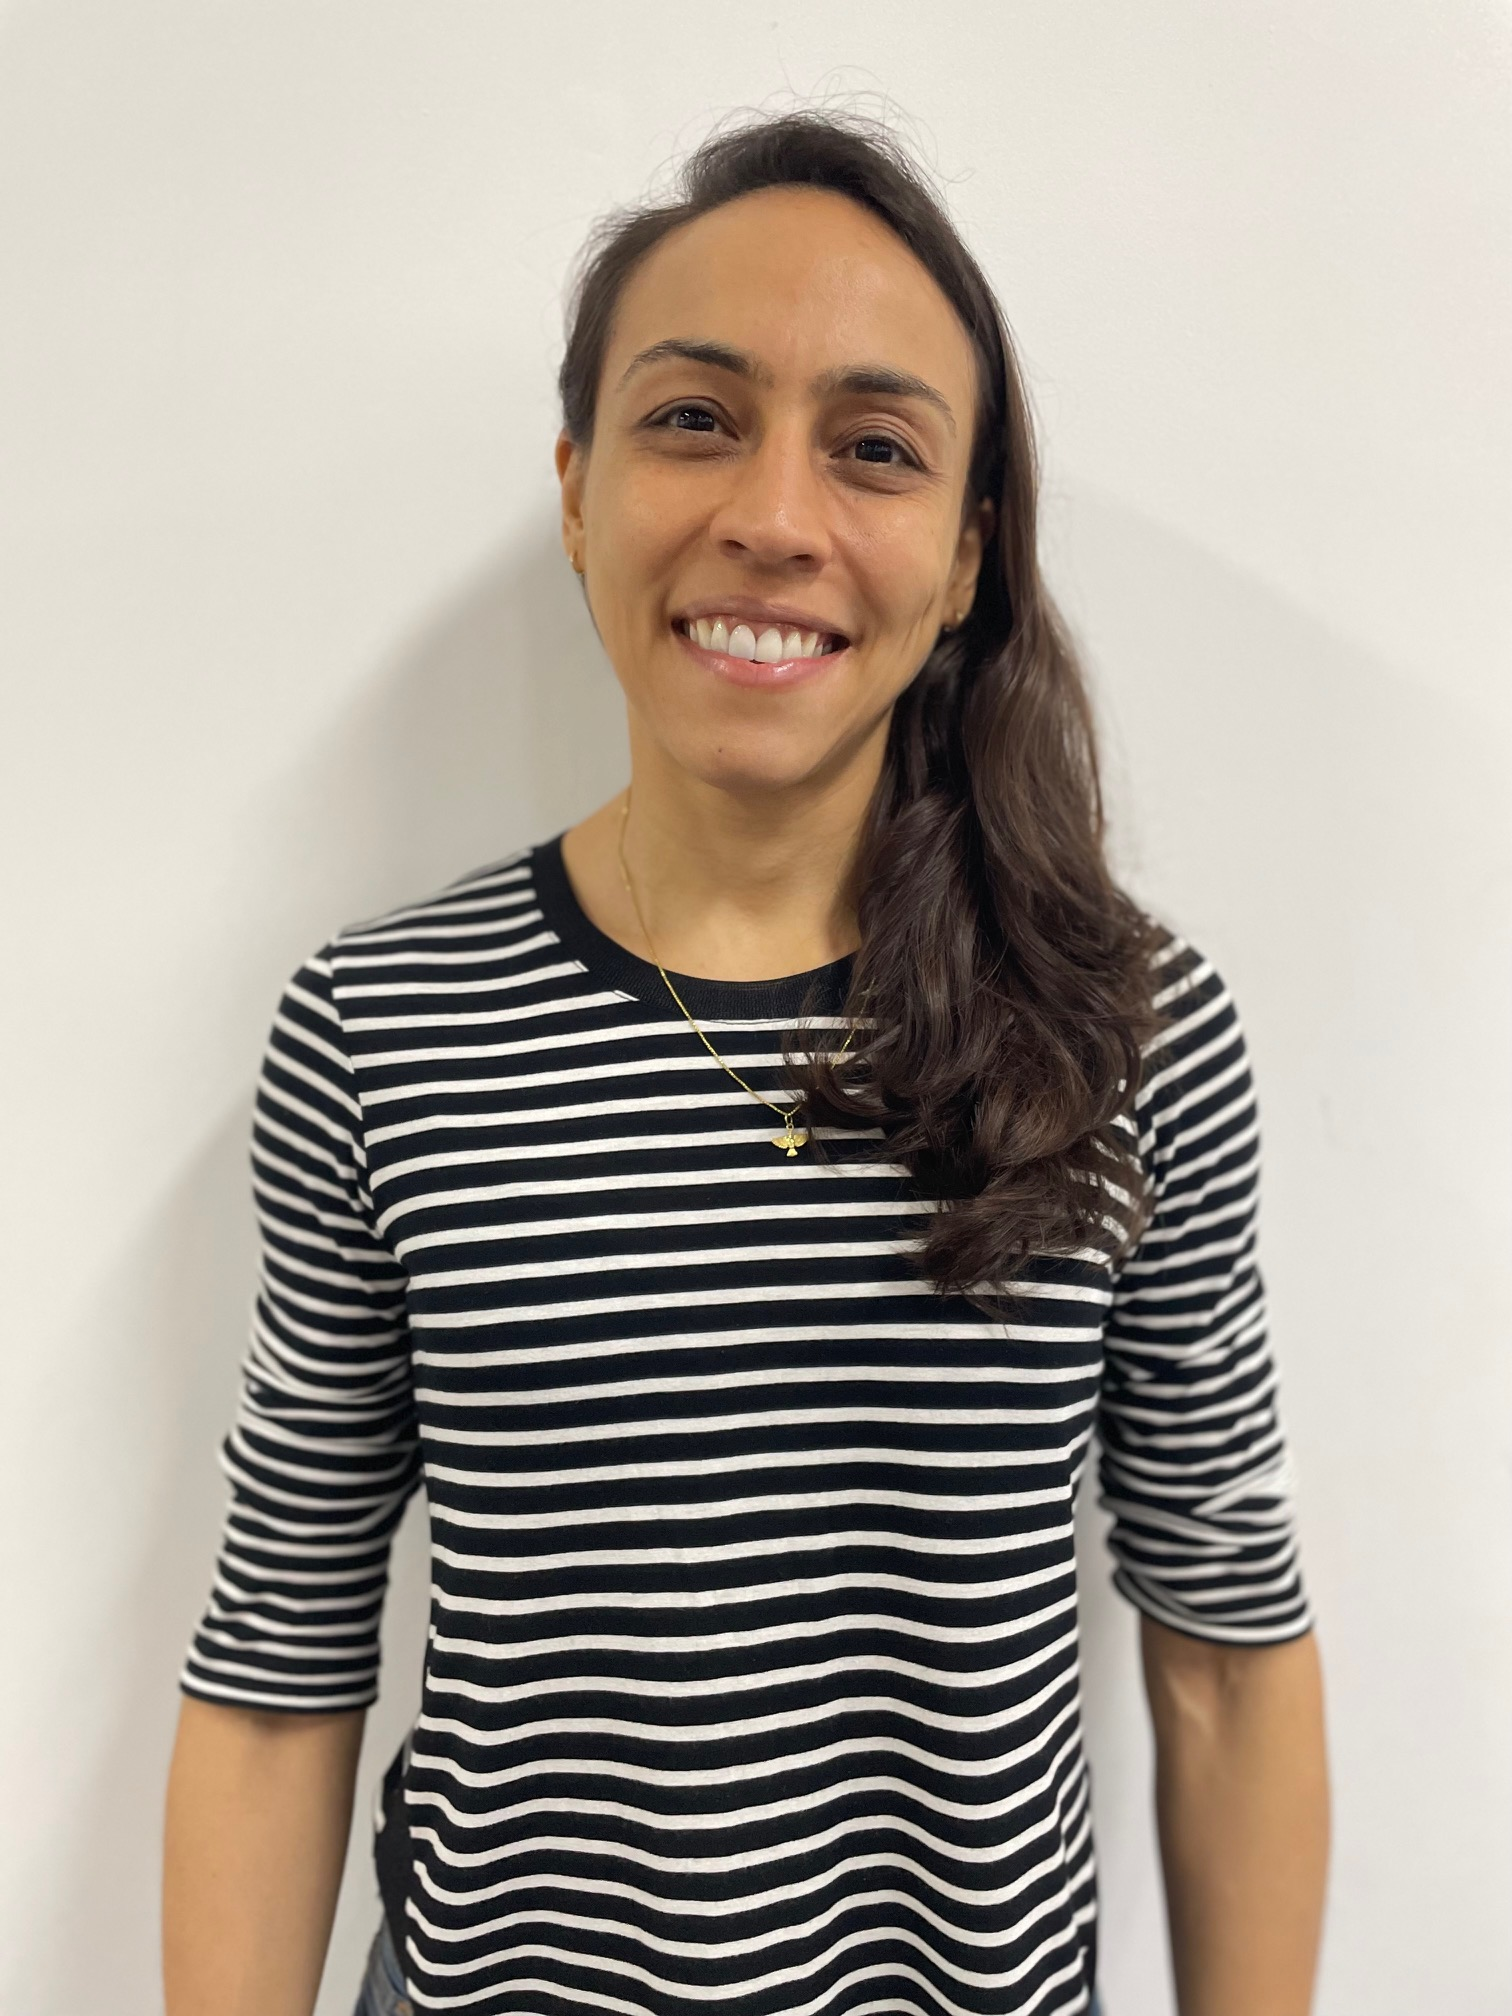
\includegraphics[width=2cm]{Elais.jpg}
\end{wrapfigure}\noindent 
Elaís Cidely é baiana, nascida na cidade de Macaúbas. Possui graduação e mestrado em matemática pela UFBA, doutorado em matemática pelo IMPA e, desde 2015, é professora do IME-UFBA. Sua área de pesquisa é Sistemas Dinâmicos, com ênfase em Teoria Ergódica. Atualmente, é coordenadora local do PICME-UFBA e vice-coordenadora institucional do PROFMAT-UFBA. Na adolescência,  tocou bateria em uma banda do colégio. Durante o doutorado, tocou alfaia em um grupo carioca de maracatu. Mas desde 2021, tem o CrossFit como parte indispensável da sua rotina.

\vspace{0.5cm}
\begin{wrapfigure}{L}{1.7cm}
	\vspace{-10pt}
	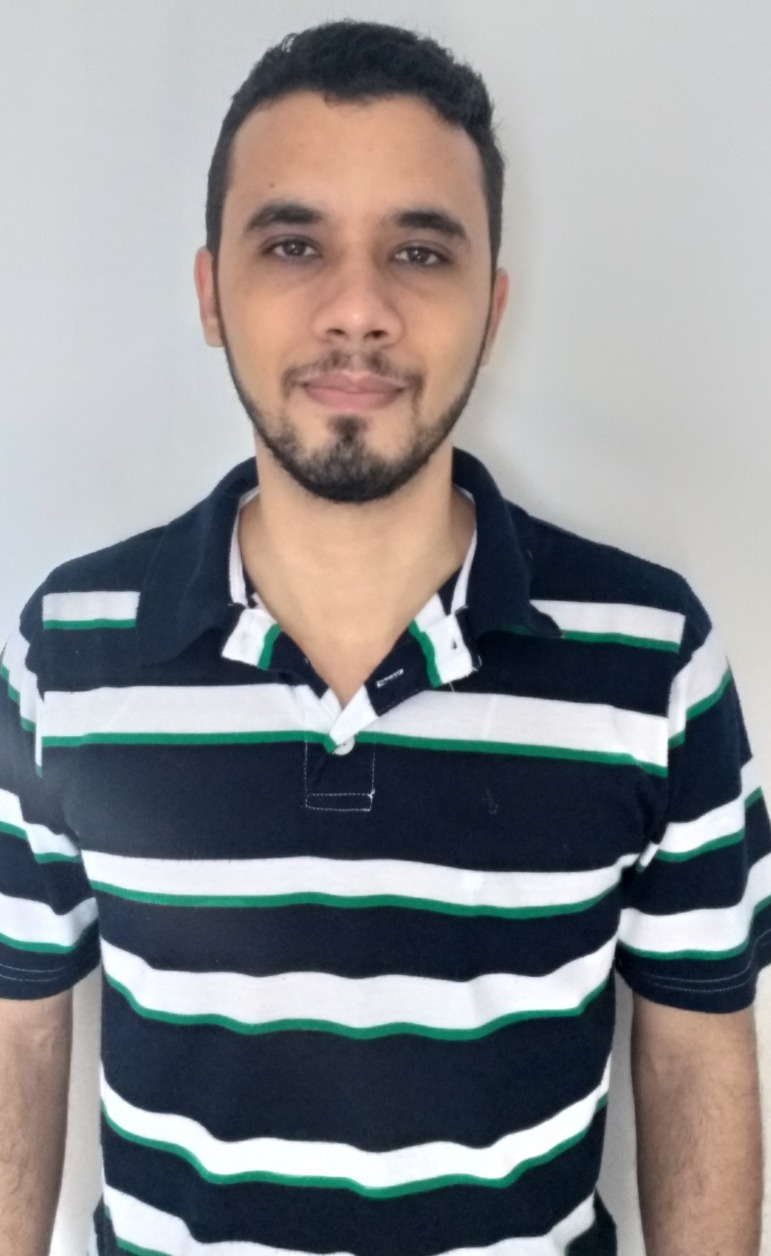
\includegraphics[width=2cm]{Roberto.JPG}
\end{wrapfigure}\noindent
  Roberto Sant'Anna é nascido e criado em Salvador, Bahia. É doutor em 
  Matemática Pura pela UFBA e atualmente é professor adjunto no Instituto 
  de Matemática Estatística da UFBA e também Coordenador Regional da OBMEP. 
  Tem realizado pesquisas na temática de Otimização Ergódica, dentro da área 
  de Sistemas Dinâmicos e também tem atuado em diversos projetos tendo em 
  vistas a divulgação da Matemática. Nas horas vagas, é amante da música e 
  busca através dela se expressar por meio do teclado ou piano, 
  instrumentos que tanto admira.





%\section{First Iteration in Dynamics}

%\section{Conclusão}



%\nocite{*}
%\bibliography{refs}

\end{document}
